\documentclass[a4paper,12pt]{article}[abnt2]
\usepackage[utf8]{inputenc} % Carrega a codificação UTF-8
\usepackage[T1]{fontenc}    % Codificação de fontes recomendada para ABNT
\usepackage{csquotes}
\usepackage[style=abnt, backend=biber]{biblatex}

\addbibresource{PEE.bib} 

\usepackage{booktabs}
\usepackage{tabularx}
\usepackage{xcolor}
\usepackage{colortbl}
\usepackage{makecell}

\usepackage{adjustbox}
\usepackage{caption}
\usepackage{subcaption}
\usepackage{float}

% Definições de layout e formatação
\usepackage[a4paper, left=3.0cm, top=3.0cm, bottom=2.0cm, right=2.0cm]{geometry} % Personalização das margens do documento
\usepackage{setspace} % Controle do espaçamento entre linhas
\onehalfspacing % Espaçamento entre linhas de 1,5
\usepackage{indentfirst} % Indentação do primeiro parágrafo das seções
\usepackage{newtxtext} % Substitui a fonte padrão pela Times Roman
\usepackage{titlesec} % Personalização dos títulos de seções
\usepackage{ragged2e} % Melhor controle de justificação do texto
\usepackage[portuguese]{babel} % Adaptação para o português (nomes e hifenização)
 \usepackage{amsmath}

% Pacotes de cabeçalho, rodapé e títulos
\usepackage{fancyhdr} % Customização de cabeçalhos e rodapés
\setlength{\headheight}{14.49998pt} % Altura do cabeçalho
\pagestyle{fancy}
\fancyhf{} % Limpa cabeçalho e rodapé
\rhead{\thepage} % Página no canto direito do cabeçalho

% Pacotes para tabelas
\usepackage{booktabs} % Melhora a qualidade das tabelas
\usepackage{tabularx} % Permite tabelas com larguras de colunas ajustáveis
\usepackage{float} % Melhor controle sobre o posicionamento de figuras e tabelas

% Pacotes para gráficos e imagens
\usepackage{graphicx} % Suporte para inclusão de imagens

\usepackage[utf8]{inputenc}
\usepackage{listingsutf8}

\lstset{
    language=R,                      
    basicstyle=\ttfamily\scalefont{1.0},
    keywordstyle=\color{blue},       
    stringstyle=\color{red},         
    commentstyle=\color{green},      
    numbers=left,                    
    numberstyle=\tiny\color{gray},   
    stepnumber=1,                    
    numbersep=5pt,                   
    backgroundcolor=\color{lightgray!10}, 
    frame=single,                    
    breaklines=true,                 
    captionpos=b,                    
    keepspaces=true,                 
    showspaces=false,                
    showstringspaces=false,          
    showtabs=false,                  
    tabsize=2,
     literate={á}{{\'a}}1
             {é}{{\'e}}1
             {í}{{\'i}}1
             {ó}{{\'o}}1
             {ú}{{\'u}}1
             {Ú}{{\'U}}1
             {â}{{\^a}}1
             {ê}{{\^e}}1
             {î}{{\^i}}1
             {ô}{{\^o}}1
             {û}{{\^u}}1
             {ã}{{\~a}}1
             {õ}{{\~o}}1
             {ç}{{\c{c}}}1,
}


% Pacotes para unidades e formatação numérica
\usepackage{siunitx} % Tipografia de unidades do Sistema Internacional e formatação de números
\sisetup{
  output-decimal-marker = {,},
  inter-unit-product = \ensuremath{{}\cdot{}},
  per-mode = symbol
}
\DeclareSIUnit{\real}{R\$}
\newcommand{\real}[1]{R\$#1}

% Pacotes para hiperlinks e referências
\usepackage{hyperref} % Suporte a hiperlinks
\usepackage{footnotehyper} % Notas de rodapé clicáveis em combinação com hyperref
\hypersetup{
    colorlinks=true,
    linkcolor=black,
    filecolor=magenta,      
    urlcolor=cyan,
    citecolor=black,        
    pdfborder={0 0 0},
}
\makeatletter
\def\@pdfborder{0 0 0} % Remove a borda dos links
\def\@pdfborderstyle{/S/U/W 1} % Estilo da borda dos links
\makeatother

% Pacotes para texto e outros
\usepackage{lipsum} % Geração de texto dummy 'Lorem Ipsum'
\usepackage[normalem]{ulem} % Permite o uso de diferentes tipos de sublinhados sem alterar o \emph{}

\begin{document}

\begin{titlepage}
    \centering
    \vspace*{1cm}
    \Large\textbf{INSPER – INSTITUTO DE ENSINO E PESQUISA}\\
    \Large ECONOMIA\\
    \vspace{1.5cm}
    \Large\textbf{Caderno}\\
    \textbf{Problemas em Economia}\\
    \vspace{1.5cm}
    Profª. Juliana Inhasz  \\
    Prof.  Sérgio Ricardo Martins \\
    Prof. Auxiliar Paulo Jose Mencacci Costa
    \vfill
    \normalsize
    Caio Santa Rosa Christovam, \href{mailto:caiosrc@al.insper.edu.br}{caiosrc@al.insper.edu.br}\\
    Érika Kaori Fuzisaka, \href{mailto:erikakf1@al.insper.edu.br}{erikakf1@al.insper.edu.br}\\
    Hicham Munir Tayfour, \href{mailto:hichamt@al.insper.edu.br}{hichamt@al.insper.edu.br}\\
    Lucas Batista Ferreira, \href{mailto:lucasbf1@al.insper.edu.br}{lucasbf1@al.insper.edu.br}\\
    Maria Antonia Pereira Guimarães, \href{mailto:mariaapg1@al.insper.edu.br}{mariaapg1@al.insper.edu.br}\\
    Maria Eduarda Marques Pereira, \href{mailto:mariaemp@al.insper.edu.br}{mariaemp@al.insper.edu.br}\\
    Maria Morais Garcia Leal, \href{mailto:mariamgl@al.insper.edu.br}{mariamgl@al.insper.edu.br}\\

    \vfill
    São Paulo\\
    Fevereiro/2025
\end{titlepage}
\newpage
\tableofcontents
\thispagestyle{empty} % Esse comando remove a numeração de pagina da tabela de conteúdo

\newpage 
\listoffigures
\thispagestyle{empty} % Esse comando remove a numeração de pagina da tabela de figura

\newpage
\listoftables
\thispagestyle{empty} % Este comando remove a numeração de página da lista de tabelas

\newpage
\setcounter{page}{1} % Inicia a contagem de páginas a partir desta página
\justify
\onehalfspacing


\section*{\textbf{Programa do Curso}}
\subsection*{\textbf{Ementa}}
Entendimento da dinâmica das variáveis econômicas. Estimação da reação destas variáveis a mudanças de política econômica ou do ambiente competitivo. Estudo de temas econômicos concretos. Papel da teoria econômica e dos métodos quantitativos no entendimento destes problemas reais.

\subsection*{\textbf{Objetivo}}
Ao final da disciplina é esperado que os alunos sejam capazes de aplicar corretamente o instrumental econômico, tanto teórico quanto estatístico, acumulado nos três primeiros anos de curso de forma a modelar e resolver problemas concretos

\subsection*{\textbf{Conteúdo Programático}}

\begin{enumerate}
    \item Câmbio, poupança e mercado de trabalho
    \item Política cambial
    \item Instrumentos alternativos de controle monetário
    \item Produtividade e mercado de trabalho
    \item Investimento
    \item Interação estratégica das firmas
    \item Teoria e comportamento do consumidor
    \item Escolha sob incerteza
\end{enumerate}

\subsection*{\textbf{Avaliações}}
\begin{itemize}
    \item \textbf{Banca 1}: 15\% da média final 
    \item \textbf{Banca 2}: 15\% da média final
    \item \textbf{Banca Final}: 20\% da média final
    \item \textbf{APS}: 5\% da média final
    \item \textbf{Checagem Obrigatória}: 10\% média final
    \item \textbf{Paper}: 35\% da média final
\end{itemize}

\section{\textbf{Apresentação da matéria "Problemas em Economia (PEE''}}
\subsection{\textbf{O que vamos fazer em PEE?}}
\begin{figure}[H]
    \centering
    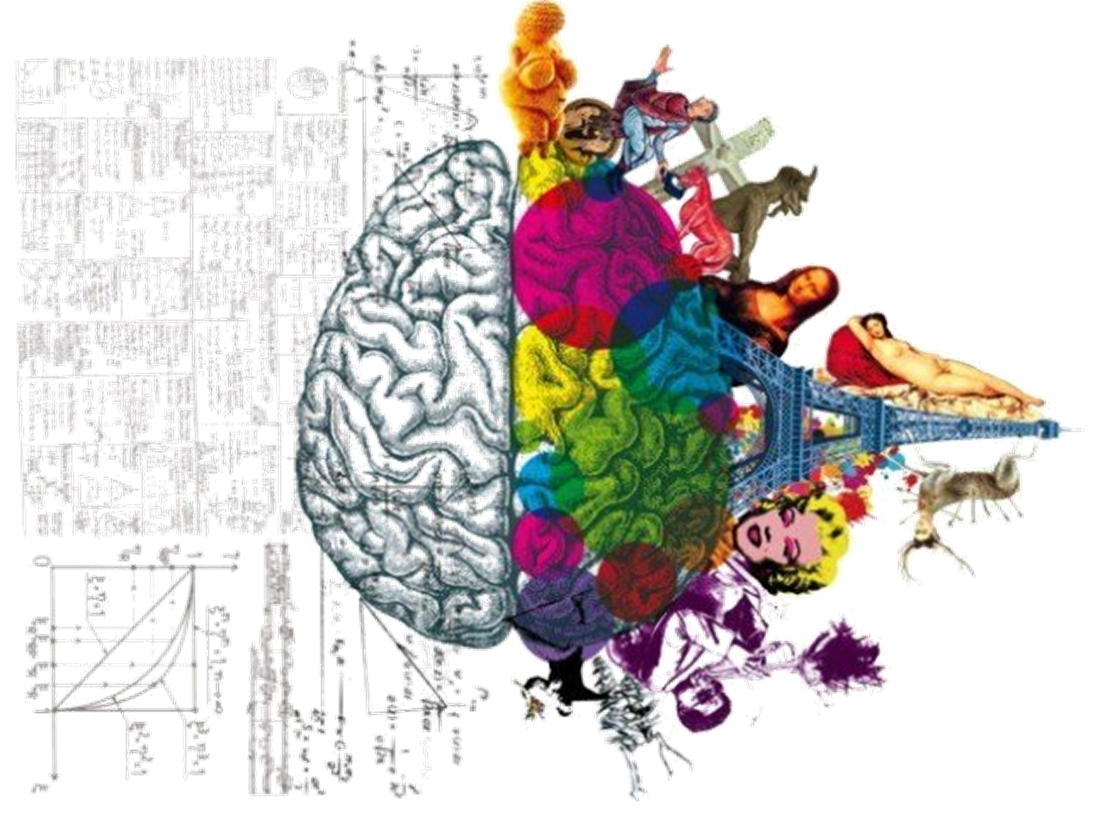
\includegraphics[width=0.5\linewidth]{Imagens/a1i1.png}
\end{figure}

Em PEE vamos resolver problemas, mas aprendendo a olhar o mundo com os olhos de economistas:\begin{enumerate}
    \item O que nos incomoda ?
    \item Quais os problemas econômicos merecem nossa maior atenção?
    \item Por que devemos pensar soluções para determinados problemas?
\end{enumerate} 

Para essa resolver problemas, precisamos de \textbf{teoria + análise empírica}, ou seja, um perfil com:\begin{itemize}
    \item Capacidade Analítica
    \item Pensamento Crítico
    \item Visão sistêmica
    \item Trabalho em equipe
    \item Comunicação
\end{itemize}

\subsection{\textbf{Estrutura do trabalho}}
\begin{figure}[H]
    \centering
    
\includegraphics[width=0.75\linewidth]{Imagens/a1i2.png}
\end{figure}

\subsection{\textbf{Entregas do Trabalho}}
\begin{figure}[H]
    \centering
    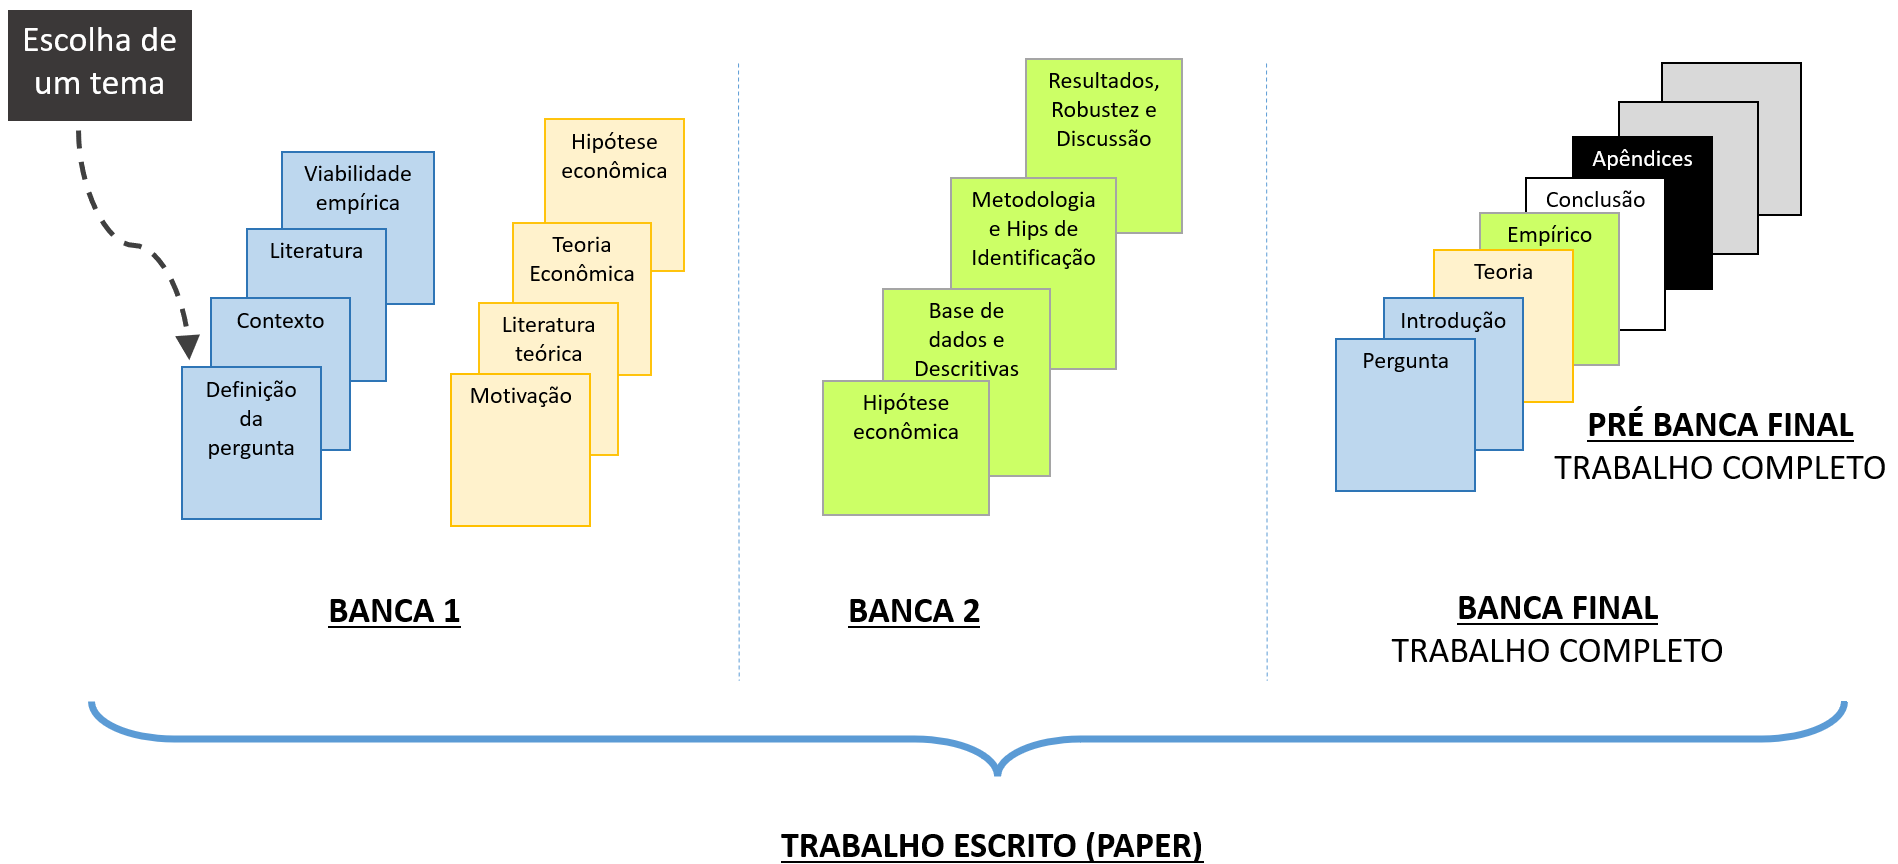
\includegraphics[width=0.75\linewidth]{Imagens/a1i3.png}
\end{figure}

\begin{enumerate}
    \item \textbf{Banca 1}: Dias 06 de Março e 10 de Março
    \item \textbf{Banca 2}: Dias 17 de Abril e 24 de Abril
    \item \textbf{Pré Banca Final}: Dias 08 de Maio e 12 de Maio
    \item \textbf{Banca Final}: Dias 19 de Maio e 22 de Maio
    \item \textbf{Trabalho Escrito (Paper)}: Dia 11 de Junho
\end{enumerate}

\subsection{\textbf{Divisão de Notas}}

Suponha um grupo com 5 integrantes. Admita que o tal grupo tenha tirado 8 em uma determinada entrega.

Dessa forma o grupo terá disponível um total de 40 pontos (5x8 = 40).  Os integrantes do grupo terão que distribuir esses pontos entre si. Em toda entrega, necessariamente, cada grupo deverá realizar a divisão de pontos. Ao final, essa nota será validada pelos professores. 

Exemplo: aluno A fica com 9, aluno B com 5, alunos C e D com 8 e aluno E com 10.

\textbf{Regra:} variância não pode ser zero (alunos não podem ter todos a mesma nota).

\subsection{\textbf{Como funcionam as APS}}

A APS será uma \textbf{avaliação sobre o conhecimento da rubrica}. Vocês receberão apresentações passadas, avaliarão e posteriormente os professores farão a correção com as notas reais, indicando como é feito o raciona para a atribuição de notas. 

A APS é \textbf{obrigatória}, feita em sala de aula, e alunos que não tiverem feito nenhuma APS são automaticamente reprovados por frequência.\begin{enumerate}
    \item \textbf{APS1}: 10/02
    \item \textbf{APS2}: 17/03
\end{enumerate} 

\subsection{\textbf{Checagens obrigatórias}}

Para que os alunos validem o seu comprometimento (ou até mesmo sua displicência com a disciplina), teremos checagens obrigatórias(\textbf{via blackboard}), espécies de pedágios onde os alunos entregarão pequenos relatórios, justificando em que ponto estão do trabalho, como estão endereçando os pontos apontados pelos professores, e como estão estruturando os próximos passos. 

Vocês deverão utilizar o aula-a-aula como guia, e devem justificar caso estejam aquém do esperado. Essas informações serão confrontadas com as anotações feitas em sala de aula, e as notas destas checagens podem ser bons preditores das eventuais notas de bancas.

Caso um (ou mais integrantes) esteja muito ausente da sala de aula, a nota do grupo nas checagens sofrerá descontos.

\begin{enumerate}
    \item \textbf{Checagem 1}: 13 de fevereiro
    \item \textbf{Checagem 2}: 24 de fevereiro
    \item \textbf{Checagem 3}: 20 de Março
    \item \textbf{Checagem 4}: 10 de Abril
    \item \textbf{Checagem 5}: 08 de Maio
\end{enumerate}

\newpage
\section{\textbf{Banca 1}}

\subsection{\textbf{Escolha do Tema}}

Considerando a importância da credibilidade do Banco Central para a condução da política monetária e seu impacto nas decisões econômicas, o grupo decidiu explorar o seguinte tema:

\textit{\textbf{A Relação entre a independência do Banco Central e a Potência da Política Monetária}}

\subsection{\textbf{Definição da Pergunta}}

A potência da política monetária está diretamente relacionada com o grau de independência institucional. No Brasil, a autonomia do Banco Central tem evoluído ao longo do tempo, influenciando a condução da política monetária e sua capacidade de ancorar expectativas e controlar a inflação. No entanto, persiste o debate sobre até que ponto a credibilidade do Banco Central impacta a potência das decisões monetárias, especialmente em cenários de instabilidade econômica.

Diante desse contexto, este estudo busca responder à seguinte questão:\begin{itemize}
    \item \textit{\textbf{Como o grau de independência do Banco Central influencia a potência da política monetária?}}
\end{itemize}


\subsection{\textbf{Contexto}}  

A independência e autonomia do Banco Central desempenham um papel determinante na eficácia (ou ``potência'') da política monetária ao influenciar a formação de expectativas e assegurar a estabilidade econômica de um país. No caso brasileiro, o grau de independência do Banco Central tem figurado como um elemento central no debate sobre a condução da política monetária, pois impacta diretamente a capacidade da autoridade monetária de controlar a inflação e, simultaneamente, estimular o crescimento econômico.

Este estudo, considerará que o conceito de independência, autonomia ou liberdade do Banco Central possuem significados equivalentes, representando a capacidade desta instituição monetária de formular e executar políticas sem interferências externas que influenciem a sua eficiência. Essa abordagem unificada permite uma análise mais objetivas dos impactos de condução da política monetária sobre a economia.

Quando o Banco Central usufrui de maior independência em relação a pressões políticas, ele tende a executar suas funções com foco no cumprimento das metas de inflação e na estabilidade do poder de compra da moeda. Esse contexto propicia uma melhor ancoragem das expectativas dos agentes econômicos, pois sinaliza compromisso firme com objetivos de longo prazo, como a estabilidade de preços. Em contrapartida, um nível insuficiente de autonomia pode gerar incertezas sobre a coerência das políticas adotadas, abrindo espaço para questionamentos quanto ao real comprometimento com a estabilidade econômica de médio e longo prazo.

Experiências internacionais e estudos empíricos sugerem que países cujos bancos centrais contam com maior independência costumam apresentar menores taxas de inflação e menor volatilidade nos indicadores macroeconômicos. No Brasil, a evolução do marco institucional que reforça a independência do Banco Central reflete a busca por um arcabouço mais robusto, no qual a decisão sobre juros, reservas internacionais e outras ferramentas monetárias seja pautada em critérios técnicos, sem depender de ciclos eleitorais ou de interesses de curto prazo.

Nesse sentido, a autonomia da autoridade monetária torna a política de taxas de juros mais previsível e diminui a possibilidade de interferências abruptas. Tal ambiente de maior credibilidade se traduz na redução do chamado \emph{prêmio de risco}, que costuma estar embutido nas taxas de juros para compensar os investidores pelas incertezas futuras. Ademais, o reforço da independência tende a diminuir a necessidade de ajustes muito bruscos da taxa de juros, contribuindo para um cenário mais estável e favorecendo tanto o planejamento de investimento das empresas quanto a gestão das finanças públicas.

É inegável, contudo, que a independência do Banco Central deve vir acompanhada de mecanismos de transparência e prestação de contas (``accountability''). Dessa forma, a sociedade e os agentes econômicos conseguem compreender os critérios técnicos que embasam as decisões de política monetária e avaliar se as metas estabelecidas estão sendo cumpridas de modo eficaz. Caso o Banco Central não seja devidamente fiscalizado ou se afaste em excesso das prioridades sociais, pode ocorrer um desalinhamento entre a condução da política monetária e outras políticas públicas, prejudicando a harmonia da gestão macroeconômica. 

Em síntese, o \textbf{grau de independência} do Banco Central influencia de modo significativo a \textbf{potência da política monetária} no Brasil ao afetar a qualidade da ancoragem de expectativas, a previsibilidade das decisões e a estabilidade dos preços. Um desenho institucional que garanta autonomia operacional para o banco emissor, aliado a mecanismos de responsabilização claros e transparentes, parece essencial para promover credibilidade, controlar a inflação e, em última análise, contribuir para um ambiente econômico mais estável e propício ao crescimento.

\subsection{\textbf{Viabilidade Empírica}}  

A análise será baseada em séries de dados macroeconômicos amplamente disponíveis, com foco em informações divulgadas por instituições públicas, como o Banco Central do Brasil (BCB), o Instituto Brasileiro de Geografia e Estatística (IBGE) e organismos internacionais. Esses dados permitirão avaliar a relação entre seu grau de independência e a potência da política monetária ao longo do tempo.  

Além disso, será necessário recorrer a indicadores \textit{proxy} que reflitam a percepção do mercado como expectativas inflacionárias, prêmios de risco e projeções de taxa de juros. Essas informações frequentemente são disponibilizadas por instituições financeiras, entidades privadas e relatórios de mercado, como o Boletim Focus do BCB.  

Para aprimorar a robustez dos estimadores e obter resultados mais consistentes, consideramos a possibilidade de utilizar variáveis macroeconômicas de outros países. A inclusão de dados internacionais permitirá a comparação de diferentes níveis de independência dos bancos centrais e seus impactos sobre a potência da política monetária.

Quanto à metodologia, reconhecemos que mensurar a influência da independência do Banco Central sobre a potência da política monetária apresenta desafios. No entanto, consideramos que sua execução é viável. O principal desafio reside na quantificação do efeito da autonomia institucional sobre variáveis como inflação, crescimento econômico e volatilidade da taxa de juros.

\subsection{\textbf{Motivação}}
O debate acerca da \textbf{independência do Banco Central} tem sido intensificado em economias emergentes como o Brasil, devido à sua relação direta com a \emph{potência da política monetária} e com a \emph{estabilidade macroeconômica} de longo prazo. Em síntese, um Banco Central autônomo tende a dispor de maior credibilidade para manter a inflação sob controle, ao passo que pressões políticas ou fiscais podem dificultar a ancoragem das expectativas inflacionárias. De acordo com \cite{adrian2024}, a adoção de novos indicadores de independência pode aprimorar a compreensão sobre quão efetiva é a autoridade monetária em um determinado arcabouço institucional.

A Figura \ref{fig:comparacao_bc} contrasta dois cenários: na Figura \ref{fig:bc_independente}, observa-se o fluxo de um Banco Central com ampla independência, resultando em maior \emph{previsibilidade} das decisões de política monetária, além de credibilidade reforçada. Já a Figura \ref{fig:bc_nao_independente} ilustra os riscos da interferência político-fiscal, elevando a \emph{volatilidade inflacionária} e minando a confiança de agentes econômicos.

\begin{figure}[H]
    \centering
    \begin{subfigure}[b]{0.45\textwidth}
        \centering
        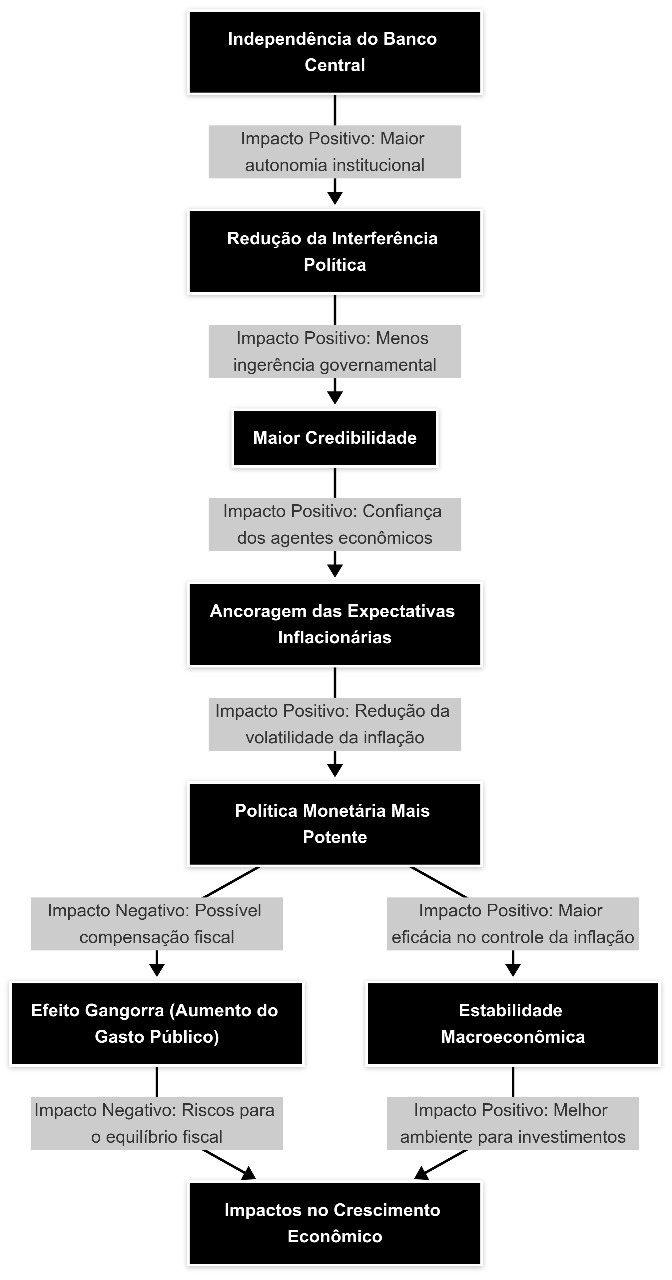
\includegraphics[width=\linewidth]{Imagens/m2i1.jpg}
        \caption{Fluxograma de um Banco Central Independente.}
        \label{fig:bc_independente}
    \end{subfigure}
    \hfill
    \begin{subfigure}[b]{0.45\textwidth}
        \centering
        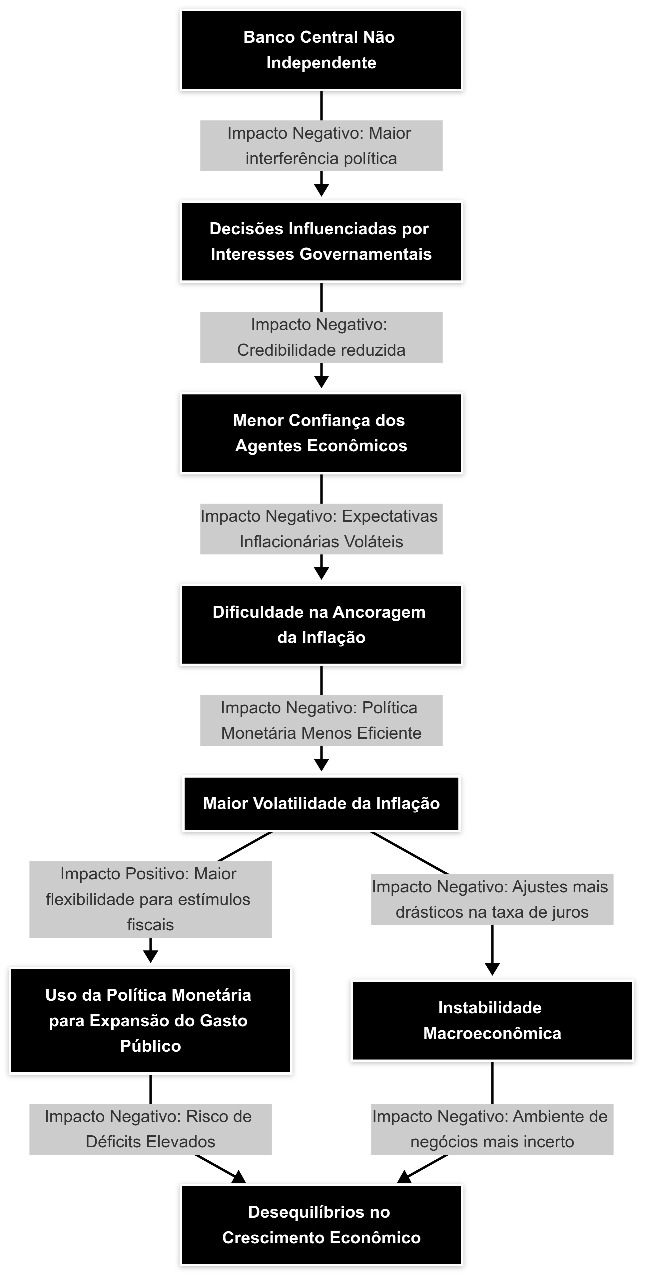
\includegraphics[width=\linewidth]{Imagens/m2i2.jpg}
        \caption{Fluxograma de um Banco Central Não Independente.}
        \label{fig:bc_nao_independente}
    \end{subfigure}
    \caption{Comparação entre Banco Central Independente e Não Independente.}
    \label{fig:comparacao_bc}
\end{figure}

O efeito de diferentes graus de autonomia sobre o controle inflacionário é evidenciado em estudos que analisam a experiência histórica de países latino-americanos. Por exemplo, \cite{jacome2022} demonstra como economias que reforçaram a independência de seus bancos centrais conseguiram atenuar episódios de hiperinflação, enquanto aquelas que não o fizeram lidaram com flutuações de preços mais severas. A Figura \ref{fig:independencepays} reflete esse ponto, exibindo a correlação negativa entre \textbf{maior independência} e \textbf{menor inflação} em países da América Latina.

\begin{figure}[H]
    \centering
    \caption{Evolução histórica da independência de Bancos Centrais e inflação na América Latina.}
    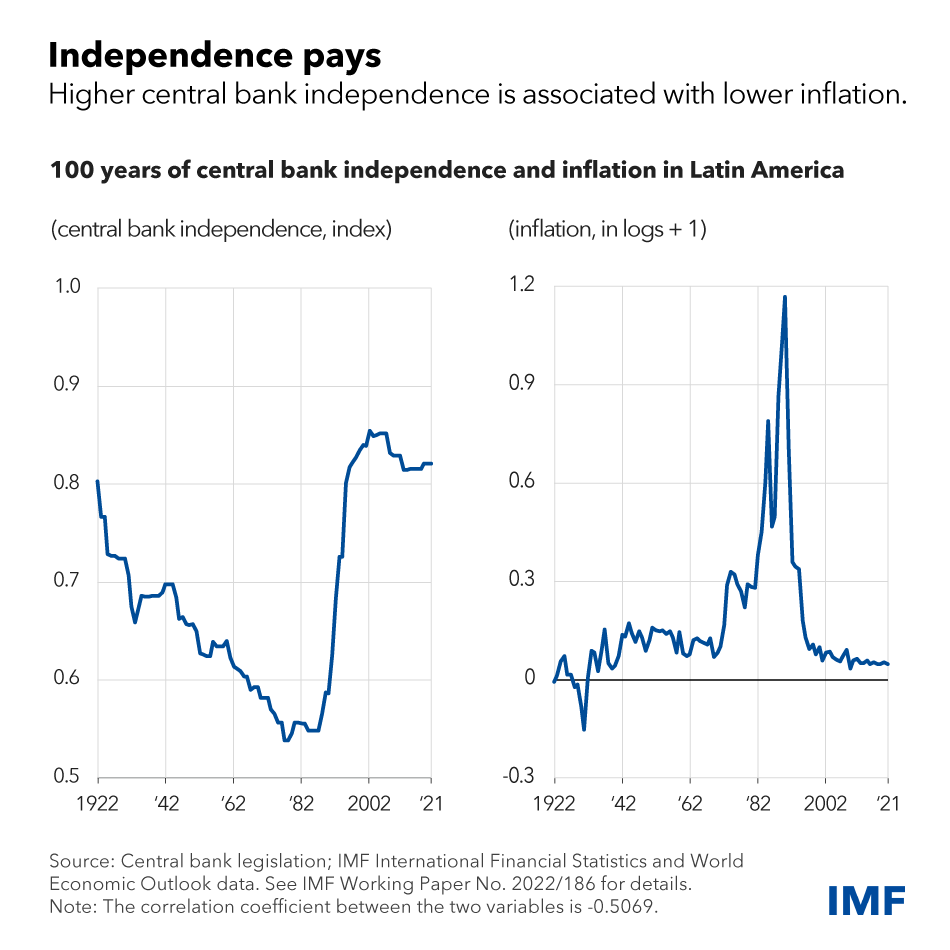
\includegraphics[width=0.7\linewidth]{Imagens/m4i1.png}
    \label{fig:independencepays}
\end{figure}

Contudo, a autonomia formal não é garantia de estabilidade macroeconômica. Conforme discutido em \cite{acemoglu2008}, \emph{reformas institucionais} podem produzir resultados díspares a depender do contexto político subjacente; assim, a ausência de mecanismos de \emph{checks and balances} pode inibir os benefícios advindos de uma autoridade monetária tecnicamente independente. Ademais, quando a independência do Banco Central reduz efetivamente a inflação, pode ocorrer o chamado \emph{efeito gangorra}, no qual o gasto público se expande, compensando as melhorias de credibilidade.

Em paralelo, \cite{unsal2023} ressalta que a força da política monetária depende não apenas das metas formais de inflação, mas também da \emph{transparência}, \emph{coerência} e \emph{consistência} com as quais o banco central comunica e implementa suas decisões. Segundo o estudo, esses pilares, aliados a um robusto \textbf{arcabouço legal}, convertem a independência de jure em \textbf{independência de fato}, reduzindo incertezas e fomentando um ambiente mais estável.

No Brasil, a adoção do \textbf{regime de metas de inflação} em 1999 trouxe a taxa Selic como principal instrumento de controle inflacionário. Contudo, a \emph{efetividade} desse regime está atrelada ao grau de autonomia do Banco Central para agir tecnicamente, de modo a ancorar as expectativas e evitar pressões políticas de curto prazo. Assim, a questão que se coloca é: \emph{em que medida o fortalecimento institucional da autoridade monetária poderia potencializar a eficácia da política de juros e, por conseguinte, aprimorar a estabilidade macroeconômica?}

A experiência internacional demonstra que a independência do Banco Central pode ser um fator essencial para garantir maior eficiência da política monetária. Países que adotaram essa autonomia mais cedo colheram benefícios como menor volatilidade inflacionária e maior credibilidade das decisões econômicas. E, apesar dessa crescente discussão, o Brasil foi o último país da América Latina a adotar a independência do Banco Central (em 2021). Esse atraso pode ter comprometido a credibilidade da política monetária ao longo de anos, sujeitando o país a episódios recorrentes de desancoragem das expectativas inflacionárias.

À luz desse debate, este trabalho pretende investigar empiricamente o \textbf{efeito da independência do Banco Central sobre a potência da política monetária no Brasil}, analisando desde o comportamento inflacionário e a trajetória histórica de reformas institucionais, até comparações com outros países da América Latina. Em última instância, busca-se compreender se a consolidação de um banco central efetivamente autônomo poderia reduzir o \emph{prêmio de risco}, reforçar a credibilidade e, desse modo, melhorar \emph{decisivamente} o cenário macroeconômico brasileiro.



\subsection{\textbf{Literatura Teórica}}
A análise sobre a independência do Banco Central (BC) e sua influência na condução da política monetária encontra respaldo em diferentes ramos da teoria econômica. Em linhas gerais, a hipótese fundamental é que a autonomia do BC mitiga problemas de inconsistência temporal e reduz incentivos para o uso político da taxa de juros, possibilitando uma melhor \emph{ancoragem das expectativas} e menor volatilidade inflacionária. No entanto, a maneira pela qual essa independência opera, bem como os resultados observados, depende tanto de variáveis institucionais quanto de aspectos político-econômicos.

\cite{adrian2024} apresentam um novo índice de independência do Banco Central, preenchendo uma lacuna na mensuração de variáveis formais e informais que moldam a autonomia das autoridades monetárias. Esse índice busca superar limitações de abordagens anteriores ao incluir dimensões como composição de diretoria, mecanismos de financiamento e até restrições à supervisão política sobre decisões de política monetária. Dessa forma, os autores propõem uma \emph{ponte} entre as características legais do arcabouço institucional e o comportamento efetivo (de facto) do BC, servindo como base empírica para estudos que examinam o grau de independência sob diferentes condições de governança e estabilidade macroeconômica.

Já \cite{jacome2022} enfatizam a importância do contexto histórico na América Latina, mostrando que choques externos e práticas políticas locais podem comprometer o sucesso de reformas que, a princípio, objetivam ampliar a autonomia do BC. Em um arcabouço dinâmico, a introdução de maior independência legal tende a produzir efeitos benéficos sobre a inflação somente se for apoiada por arranjos institucionais confiáveis e \emph{checks and balances} robustos. Em contrapartida, países com históricos recorrentes de instabilidade política ou hiperinflação podem enfrentar obstáculos ao implementar reformas, pois essas mudanças podem ser revertidas ou esvaziadas pela ação de grupos políticos poderosos.

Em consonância, \cite{unsal2023} defendem a análise da independência do Banco Central a partir de múltiplas dimensões, como \emph{accountability}, \emph{estratégia operacional} e \emph{transparência}. Esses elementos estariam diretamente associados à eficácia do BC na condução de um regime de metas de inflação, particularmente em economias emergentes. Nesse sentido, o compromisso crível com o controle de preços requer tanto a formalização de metas quantitativas claras quanto a consolidação de práticas transparentes de divulgação de dados e justificativas das decisões de juros. Esses fatores reforçam um ambiente em que o BC passa a ser avaliado pelo seu \emph{desempenho} e não apenas pela sua estrutura legal.

Por outro lado, a literatura de viés político-econômico, notadamente em \cite{acemoglu2008}, alerta que a concessão de independência monetária não implica, necessariamente, em melhores resultados. Os autores sugerem que \emph{restrições institucionais fracas} podem levar à anulação dos efeitos positivos, pois o mesmo governo que concede autonomia ao BC pode alocar gastos públicos de forma desordenada (efeito gangorra), neutralizando a redução da inflação por meio de desequilíbrios fiscais. Além disso, \cite{acemoglu2008} discutem como os benefícios da independência são mais visíveis quando há um nível de “restrições intermediárias”: a autonomia monetária tende a produzir impactos significativos em países cuja governança não é absolutamente consolidada, mas que dispõem de mecanismos mínimos de fiscalização e responsabilização política.

\subsubsection{\textbf{Ponte para o Modelo Econômico}}
A partir desses elementos teóricos, pode-se estruturar um \emph{modelo econômico} de inspiração Novo-Keynesiana, no qual a autoridade monetária define a taxa de juros segundo uma \textbf{Regra de Taylor} ampliada pela variável de independência. Nesse arranjo, a \textbf{função perda do Banco Central} é minimizada ao equilibrar a inflação e o desvio do produto em relação a seu nível potencial; quanto maior a independência, maior a ênfase em manter a inflação estável sem interferências políticas. Entretanto, a credibilidade do BC, crucial para a \emph{ancoragem das expectativas}, depende das condições institucionais: se houver mecanismos de enforcement de longo prazo (como discutido em \cite{jacome2022,acemoglu2008}), o banco central obterá maior sucesso em evitar que choques externos ou demandas populistas resultem em inflação cronicamente elevada.

Dessa forma, a literatura teórica oferece uma base consistente para a análise empírica. O presente estudo se beneficiará das contribuições de \cite{adrian2024}, \cite{jacome2022}, \cite{unsal2023} e \cite{acemoglu2008} ao incorporar, no modelo econômico, aspectos institucionais, histórico-regulatórios e políticos que interagem com a \emph{independência do Banco Central} e influenciam, em última instância, a \emph{potência da política monetária} no Brasil.

\subsection{\textbf{Teoria Econômica}}

Para analisar a relação entre \textbf{independência do Banco Central} e \textbf{política monetária}, é útil adotar um \emph{modelo Novo-Keynesiano} como estrutura básica, pois este tipo de modelo enfatiza a importância das \emph{expectativas} e da \emph{consistência temporal} na determinação dos níveis de inflação e produto. Na essência, o modelo contempla duas equações principais: a \textbf{Curva de Phillips Novo-Keynesiana} e a \textbf{Equação IS}, que descrevem, respectivamente, a evolução da inflação e a dinâmica da demanda agregada.

\subsubsection{\textbf{Curva de Phillips Novo-Keynesiana (NKPC)}}
A Curva de Phillips Novo-Keynesiana pode ser expressa da seguinte forma:

\begin{equation}
\pi_t = \beta \, E_t[\pi_{t+1}] + \kappa \, (y_t - y_t^*) + \epsilon_t,
\end{equation}

onde $\pi_t$ representa a taxa de inflação no período $t$, $E_t[\pi_{t+1}]$ denota as expectativas de inflação futura, $\beta$ é o fator de desconto intertemporal, $\kappa$ é um parâmetro que mede o grau de rigidez de preços e $\epsilon_t$ é um choque de oferta. O termo $(y_t - y_t^*)$ indica o \emph{hiato do produto} (diferença entre o produto efetivo e o produto potencial), que afeta a inflação através de pressões de demanda. Estudos como \cite{unsal2023} destacam a relevância dessa estrutura, pois ela enfatiza que a \emph{credibilidade} do Banco Central influencia $E_t[\pi_{t+1}]$, e, portanto, o \emph{trade-off} entre estabilização do produto e controle inflacionário.

\subsubsection{\textbf{Equação IS e Política Monetária}}
A demanda agregada é frequentemente modelada através de uma \textbf{equação IS}, que relaciona o \emph{desvio do produto} às decisões de política monetária e às expectativas:

\begin{equation}
y_t - y_t^* = E_t[y_{t+1} - y_{t+1}^*] - \phi \, \big( i_t - E_t[\pi_{t+1}] - r_t^* \big) + \eta_t,
\end{equation}

onde $i_t$ é a taxa de juros nominal definida pela autoridade monetária, $E_t[\pi_{t+1}]$ representa a expectativa de inflação futura, $r_t^*$ é a \emph{taxa de juros real de equilíbrio} e $\eta_t$ é um choque de demanda. O parâmetro $\phi > 0$ mede a sensibilidade da demanda a variações na taxa de juros real. Esse arcabouço evidencia como a decisão de juros do Banco Central impacta a atividade econômica, bem como a formação de expectativas, permitindo examinar em que medida a \textbf{independência da autoridade monetária} se traduz em maior eficácia na estabilização do ciclo econômico.

\subsubsection{\textbf{Regra de Política Monetária e Independência}}
A \textbf{Regra de Taylor} é amplamente utilizada para descrever como o Banco Central ajusta sua taxa de juros em resposta a desvios da inflação em relação à meta e a variações do produto em relação ao seu potencial:

\begin{equation}
i_t = \rho \, i_{t-1} + (1 - \rho) \big[ r_t^* + \pi_t + \alpha (\pi_t - \pi^*) + \gamma (y_t - y_t^*) \big] + \nu_t,
\end{equation}

em que $\pi^*$ é a meta de inflação e $\nu_t$ corresponde a um choque de política monetária. O parâmetro $\rho \in [0,1]$ reflete o grau de \textbf{suavização} da taxa de juros, enquanto $\alpha$ e $\gamma$ medem a intensidade da reação do Banco Central aos desvios da inflação e do produto, respectivamente. Em um contexto de \emph{independência monetária}, espera-se que a instituição conduza sua política de maneira a minimizar o impacto de pressões políticas de curto prazo, focando no objetivo de estabilizar a inflação e reduzir volatilidades excessivas do ciclo econômico \cite{adrian2024,woodford2003, unsal2023, gali2015}.

\subsubsection{\textbf{Mecanismo de Independência e Credibilidade}}
O elo entre \textbf{independência} do Banco Central e \textbf{credibilidade} torna-se mais claro quando se introduz uma \emph{função de perda} para a autoridade monetária. Geralmente, assume-se que o Banco Central procura minimizar:

\begin{equation}
\mathcal{L} = \sum_{t=0}^{\infty} \beta^t \left[ (\pi_t - \pi^*)^2 + \lambda (y_t - y_t^*)^2 \right],
\end{equation}

onde $\lambda \ge 0$ pondera a importância relativa que o BC atribui a flutuações do produto\cite{woodford2003, unsal2023, gali2015}. Em cenários de elevada independência, a autorresponsabilização pelas metas de inflação e a redução de interferências governamentais fortalecem a credibilidade da instituição, ancorando expectativas de forma mais eficiente \cite{jacome2022}. Entretanto, caso haja \emph{mecanismos institucionais fracos} ou oscilações políticas recorrentes, a independência formal pode não se traduzir em independência de fato, produzindo resultados aquém do potencial \cite{acemoglu2008}.

\subsubsection{\textbf{Ramificações Institucionais}}
A literatura destaca que a \emph{consistência temporal} constitui o principal pilar teórico que justifica a independência: governos tendem a ter incentivos a usar a política monetária para estimular a economia antes de eleições ou para financiar gastos via senhoriagem. Quando o BC não é independente, há o risco de \emph{inconsistência dinâmica}, resultando em inflação mais alta \cite{acemoglu2008}. Além disso, estudos como \cite{jacome2022} mostram que, em países latino-americanos, a credibilidade do BC sofre com frequentes mudanças legislativas e interferências do Executivo, evidenciando as \textbf{ramificações político-institucionais} do modelo teórico: a capacidade de o BC conduzir a política monetária de forma ótima depende da solidez do \emph{arcabouço de governança} que garante sua autonomia.

Finalmente, \cite{unsal2023} sustentam que a \textbf{transparência}, a \textbf{accountability} e a \textbf{consistência de metas} ampliam a eficácia do Banco Central. Dessa forma, a \emph{independência} deve ser acompanhada de mecanismos que incentivem a disciplina fiscal, reduzam a opacidade na comunicação da política monetária e aperfeiçoem o \emph{compliance} do banco central com suas metas. Em síntese, o modelo econômico proposto incorpora a interação entre \textbf{estrutura legal}, \textbf{regras de política}, \textbf{expectativas racionais} e \textbf{contexto político}, formando uma ponte entre a teoria Novo-Keynesiana e a evidência empírica sobre a relevância da independência monetária. 

\subsubsection{\textbf{Expectativas de Inflação Ancoradas}}
\begin{equation}
\pi_t^E = \chi \pi^T + (1 - \chi)\pi_{t-1}
\end{equation}
\noindent Onde $\chi$ representa o grau de ancoragem das expectativas: quanto mais próximo de 1, mais ancoradas na meta de inflação $\pi^T$ estão as expectativas dos agentes.

\subsubsection{\textbf{Curva de Phillips com expectativas ancoradas}}
\begin{equation}
\pi_t = \pi_t^E + \alpha (y_t - y^e)
\end{equation}
\noindent A inflação depende das expectativas e do hiato do produto. A ancoragem das expectativas influencia diretamente na persistência inflacionária.

\subsubsection{\textbf{Função de perda do Banco Central}}
\begin{equation}
L = (y_t - y^T)^2 + \beta(CBI) \cdot (\pi_t - \pi^T)^2
\end{equation}
\noindent Essa função mede o "custo social" das flutuações econômicas. Onde $\beta(CBI)$ reflete o peso relativo dado à estabilidade de preços, condicionado pelo grau de independência do Banco Central ($CBI$):
\begin{equation}
\beta(CBI) = \beta_0 + \beta_1 \cdot CBI, \quad \beta_1 > 0
\end{equation}

\subsubsection{\textbf{Regra ótima de política monetária}}
A partir da minimização da função de perda, obtemos:
\begin{equation}
y_t - y^T = - \alpha \cdot \beta(CBI) \cdot (\pi_t - \pi^T)
\end{equation}
\noindent  Quanto maior o valor de $\beta(CBI)$, mais agressivamente o BC responde aos desvios inflacionários.

\subsubsection{\textbf{Curva IS e a Função de Reação do Banco Central}}
Consideramos a curva IS:
\begin{equation}
y_t = \bar{a} - \sigma (r_t - r^n)
\end{equation}
\noindent Substituindo na equação de reação otimizada, temos:
\begin{equation}
r_t = r^n + \frac{1}{\sigma}(\bar{a} - y^T + \alpha \beta(CBI)(\pi_t - \pi^T))
\end{equation}
\noindent Assim, a versão da regra de Taylor implícita do modelo revela o fator de reação:
\begin{equation}
\phi_\pi = \frac{\alpha \cdot \beta(CBI)}{\sigma}
\end{equation}
\noindent Ou seja, o BC ajusta a taxa de juros proporcionalmente ao desvio inflacionário, com intensidade crescente à medida que $\beta(CBI)$ aumenta.

\subsubsection{\textbf{Potência da política monetária}}
A potência é definida como a sensibilidade da inflação à taxa de juros:
\begin{equation}
\text{Potência} = \left| \frac{\partial \pi_t}{\partial r_t} \right| = \frac{\sigma}{\alpha \cdot \beta(CBI)}
\end{equation}
\noindent Portanto, maior $\beta(CBI)$ $\Rightarrow$ menor variação da inflação por unidade de taxa de juros $\Rightarrow$ maior potência monetária (efeito mais eficiente).

\subsubsection{\textbf{Conclusão}}
Este modelo mostra que a independência do Banco Central influencia diretamente o peso dado à estabilidade de preços (via $\beta$), o que se traduz em uma reação mais agressiva à inflação (via $\phi_\pi$), aumentando a potência da política monetária. A ancoragem das expectativas ($\chi$) também reforça esse canal, ao reduzir a persistência inflacionária. Assim, maior independência implica maior credibilidade, maior reação e maior potência de controle da inflação.


\subsection{\textbf{Hipótese Econômica}}

Derivado do arcabouço teórico apresentado e das evidências empíricas discutidas na literatura \cite{adrian2024, jacome2022, unsal2023, acemoglu2008, woodford2003, gali2015}, propõe-se a seguinte hipótese central:

\begin{quote}
\textit{``Quanto maior o grau de independência do Banco Central, maior será a potência da política monetária no controle inflacionário.''}
\end{quote}

Em termos \textbf{operacionais}, essa hipótese se desdobra em três pontos específicos que podem ser \emph{testados empiricamente}:

\begin{enumerate}
    \item \textbf{Efeito sobre a inflação e volatilidade inflacionária:} \\
    Países (ou períodos) com maior independência do Banco Central tendem a exibir taxas de inflação mais baixas e menor volatilidade de preços, controlando por variáveis macroeconômicas fundamentais (por exemplo, nível de desenvolvimento, regime cambial e choques externos).

    \item \textbf{Ancoragem de expectativas:} \\
    Uma autoridade monetária independente, ao sinalizar compromisso crível com a estabilidade de preços, contribui para a redução das expectativas inflacionárias de longo prazo, capturadas em medidas de \emph{survey} ou \emph{yields} de títulos indexados.

    \item \textbf{Interação com restrições institucionais:} \\
    A relação positiva entre autonomia do BC e estabilidade de preços é mais forte em países que contam com \emph{checks and balances} suficientes para evitar o chamado \emph{efeito gangorra} \cite{acemoglu2008}, ou seja, quando não há expansão fiscal compensatória que anule os ganhos de credibilidade da autoridade monetária.
\end{enumerate}

\noindent
\textbf{Teste Implementável.} Para avaliar empiricamente a hipótese, propõe-se:
\begin{itemize}
    \item \textbf{Construir ou utilizar um índice de independência do Banco Central} (como o de \cite{adrian2024} ou outro disponível em bases internacionais), que mensure não apenas aspectos legais, mas também dimensões práticas da autonomia.
    \item \textbf{Regressões econométricas} em painel ou \emph{cross-country}, onde a variável dependente pode ser a \emph{taxa de inflação}, \emph{volatilidade inflacionária} ou \emph{indicadores de estabilidade macroeconômica}. As variáveis explicativas incluem o índice de independência, controles macroeconômicos (crescimento do PIB, abertura comercial, regime cambial etc.) e indicadores de qualidade institucional.
    \item \textbf{Possível abordagem de interação:} introduzir um termo de interação entre o índice de independência do BC e um indicador de restrições institucionais ou governança (por exemplo, \emph{executive constraints}), verificando se o efeito benéfico da independência é amplificado ou atenuado em regimes institucionais diferentes \cite{acemoglu2008}.
\end{itemize}

Em síntese, a hipótese estabelecida permite relacionar diretamente as \emph{implicações do modelo Novo-Keynesiano} (focado em expectativas e consistência temporal) com o \emph{papel institucional} de um Banco Central autônomo. Essa abordagem viabiliza um teste empírico robusto, capaz de aferir se a independência monetária se traduz em maior controle da inflação, bem como se tal relação depende de fatores político-institucionais que reforcem ou inibam o efeito desejado.

\newpage
\section{\textbf{Banca 2}}
\subsection{\textbf{Hipótese Econômica}}
A hipótese econômica formulada pelo grupo foi:

\textit{"Quanto maior o grau de independência do Banco Central, maior será a potência da política monetária no controle inflacionário"}

\subsection{\textbf{Base de dados e Descritivas}}

A base de dados utilizada neste estudo foi construída a partir da integração de diversas fontes, com ênfase nos dados provenientes do Fundo Monetário Internacional (FMI), do World Development Indicators (WDI) ,do CBIdata, do The Global Economy, Eiko(LSEG) e MacroBond. As bases foram coletadas e organizadas para permitir uma análise econômica e institucional aprofundada de múltiplos países ao longo do tempo.

\subsubsection{\textbf{Dados do FMI e do WDI}}
Os dados macroeconômicos essenciais foram extraídos utilizando duas importantes bibliotecas do R:
\begin{itemize}
    \item \textbf{World Development Indicators (WDI)}: Através da biblioteca \texttt{WDI} \cite{WDI}, foram baixadas séries históricas de variáveis fundamentais, tais como o Produto Interno Bruto (PIB) Real, inflação e dívida, iniciando em 1960. Esse processo envolveu o uso dos pacotes \texttt{tidyverse} \cite{tidyverse} e \texttt{countrycode} \cite{countrycode} para filtrar e padronizar os dados, excluindo agrupamentos regionais que não eram pertinentes à análise. Fonte: \url{https://data.worldbank.org/indicator}.
    \item \textbf{Fundo Monetário Internacional (FMI)}: Utilizando a biblioteca \texttt{imf.data} \cite{imf.data}, foram obtidas séries históricas referentes à política monetária, como as taxas de juros dos bancos centrais, com dados disponíveis em periodicidade anual para o período de 1960 a 2025. Ressalta-se que o FMI funciona como um repositório de dados originalmente reportados por fontes nacionais e internacionais. Fonte: \url{https://data.imf.org}.
\end{itemize}

\subsubsection{\textbf{Dados do CBIdata}}
A base do CBIdata foi construída a partir de uma planilha em Excel que contém os índices de independência dos bancos centrais, fundamentais para mensurar a autonomia das instituições monetárias em relação ao governo. Esses índices, que incluem o índice CBIE de Romelli (2022, 2024) e os índices clássicos de Grilli, Masciandaro e Tabellini (1991) e de Cukierman, Webb e Neyapti (1992), foram extraídos de legislações e documentos oficiais dos bancos centrais. Para a importação desta planilha, foi utilizada a biblioteca \texttt{readxl} \cite{readxl}. Essa fonte permite explorar a relação entre a independência dos bancos centrais e as principais variáveis macroeconômicas, como inflação e crescimento econômico. Fonte: \url{https://cbidata.org/}.

\subsubsection{\textbf{Dados de Expectativas de Inflação}}

A base \texttt{InflationForecast (FMI)} foi extraída do site \texttt{TheGlobalEconomy.com}, que agrega projeções de inflação calculadas pelo FMI. As expectativas de inflação são fundamentais para o modelo ecônomico, dado que na Curva de Phillips Novo-Keynesiana (NKPC) ela é um componente fundamental para formulação da inflação. Fonte: \url{https://www.theglobaleconomy.com/}

\subsubsection{\textbf{Dados de Meta de Inflação}}

A base \texttt{taget(Eikon)} e \textit{taget(MacroBond)} agregametas de inflação divulgadas pelos Bancos Centrais de cada país |(que tem meta de inflação). As metas de inflação são fundamentais para o modelo ecônomico, dado que na Curva de Phillips Novo-Keynesiana (NKPC) ela é um componente fundamental para formulação da inflação. 

Essa abordagem integrada, com o uso extensivo das bibliotecas \texttt{WDI} \cite{WDI} e \texttt{imf.data} \cite{imf.data} para a extração e padronização dos dados, e a elaboração cuidadosa do dataframe de metas de inflação, possibilitou a criação de uma base robusta e detalhada. Tal base é capaz de sustentar análises comparativas entre diferentes períodos e regiões, contribuindo para uma compreensão mais aprofundada das dinâmicas econômicas e institucionais dos países analisados.

\subsection{\textbf{Estrutura da base e cobertura dos dados}}

A amostra consiste em um \textbf{painel país–ano} cobrindo \textbf{78 países}, no período de \textbf{2000 a 2023}. Essa estrutura permite analisar, simultaneamente, variações \emph{entre} países (por exemplo, diferentes graus de independência do banco central – \emph{CBI}) e \emph{ao longo do tempo} dentro de cada país.

\begin{figure}[H]
    \centering
    \caption{Cobertura de dados por país e variável}
    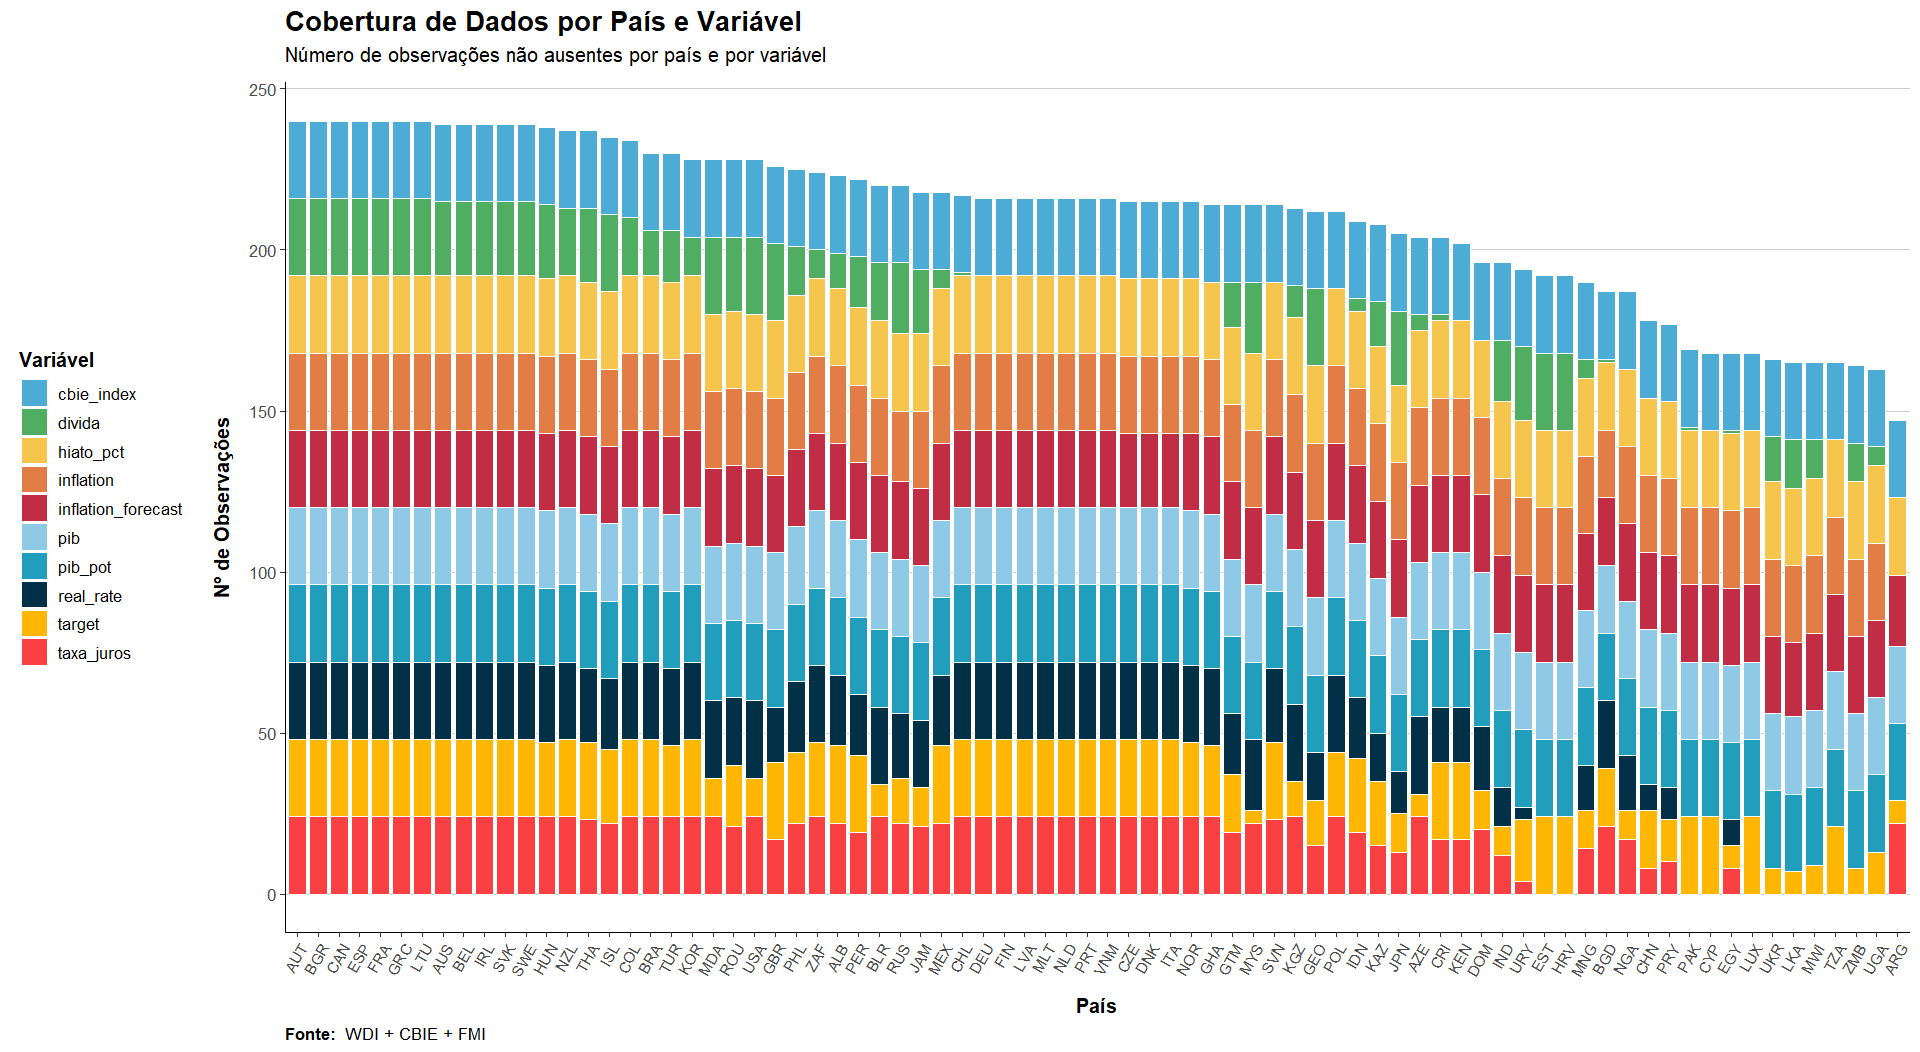
\includegraphics[width=.85\linewidth]{Imagens/an1i1.png}
    \caption*{\footnotesize Cada barra empilhada indica o número de observações não ausentes (máx.\ = 24) para cada variável em cada país.}
\end{figure}

\begin{figure}[H]
    \centering
    \caption{Proporção de dados observados por país (2000–2023)}
    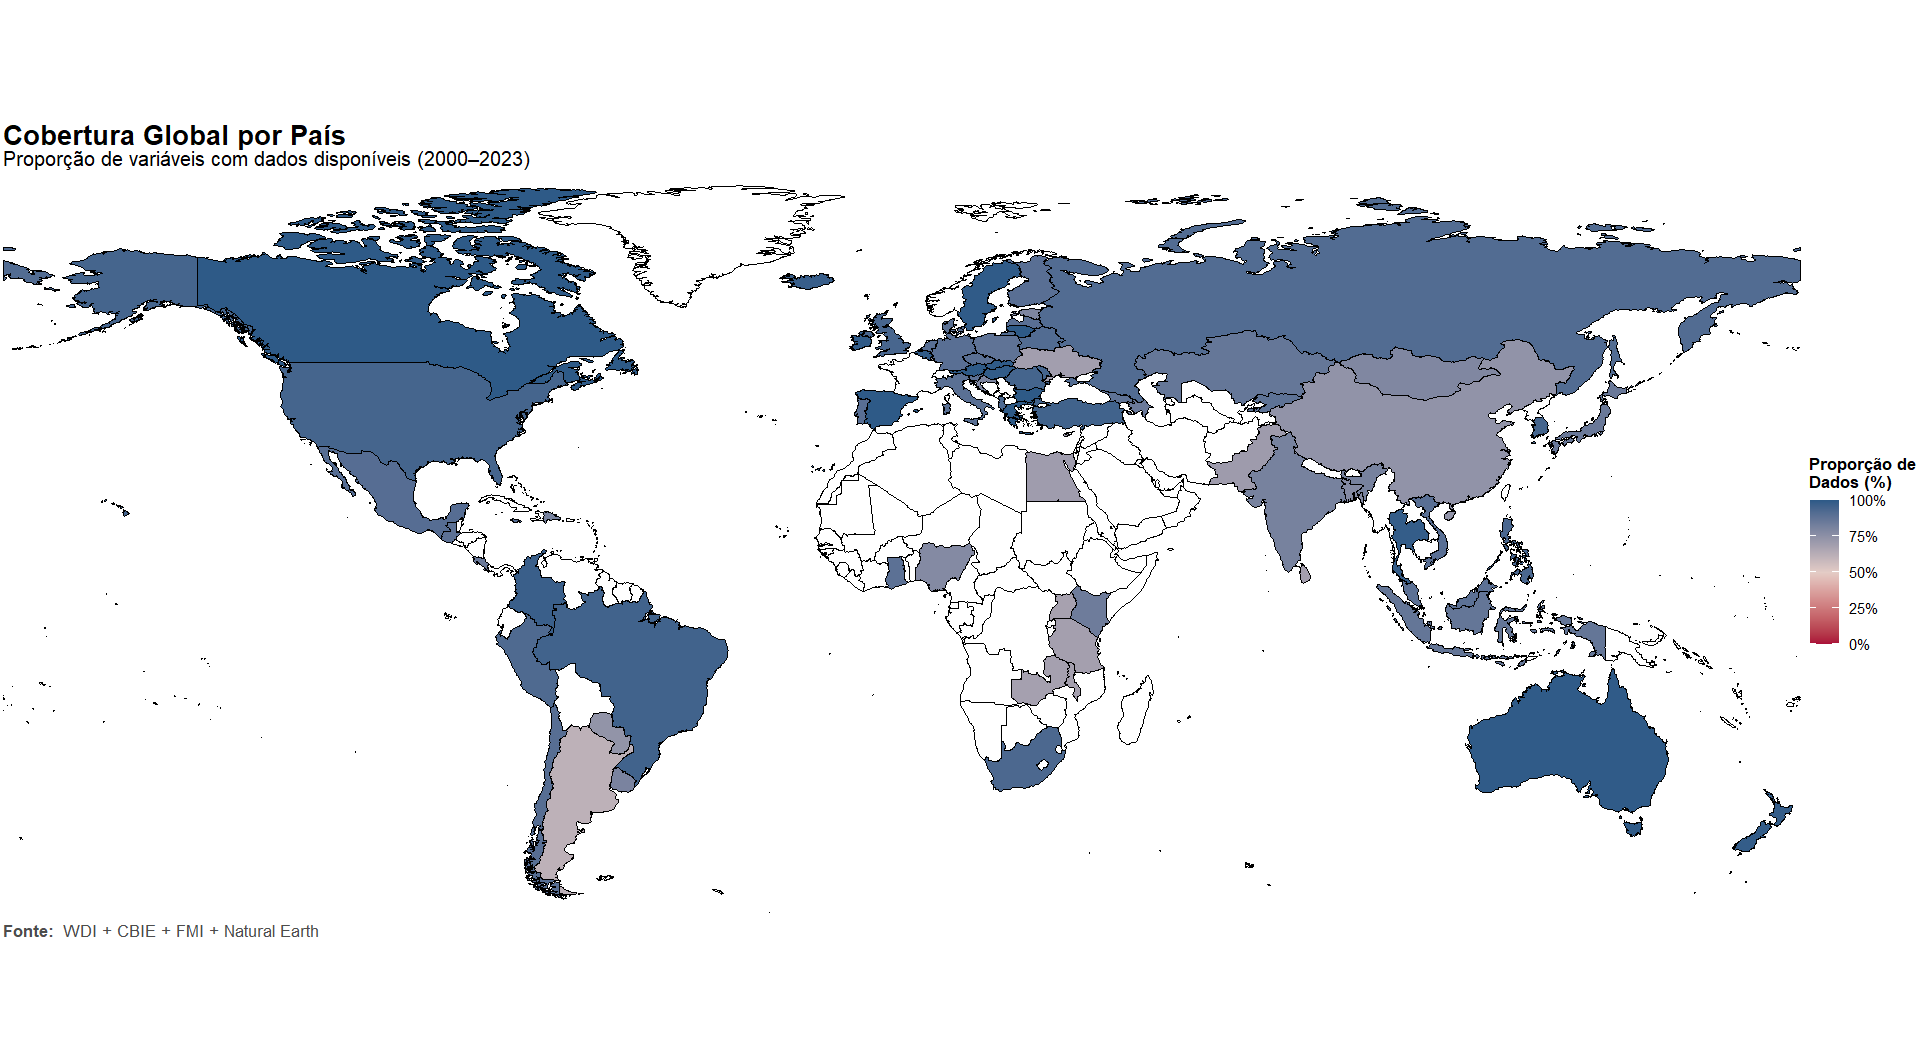
\includegraphics[width=.85\linewidth]{Imagens/an1i2.png}
    \caption*{\footnotesize Tons mais escuros indicam maior completude; países claros exigem cautela na interpretação dos efeitos.}
\end{figure}

\vspace{.5em}
\noindent\textit{Leitura inicial.}  

(i) O \emph{CBI Index} apresenta ampla cobertura, sustentando sua inclusão no modelo;  

(ii) há lacunas na série de dívida pública e na taxa de juros, o que sugere o uso de estimadores robustos a painéis desbalanceados;  

(iii) a amostra engloba todas as regiões do FMI, mitigando possíveis vieses de seleção.

\begin{table}[H]
\centering
\small
\caption{Completude das variáveis da base (máx.\ = 1872 observações)}
\label{tab:base_dados}
\setlength{\tabcolsep}{4pt}
\begin{tabular}{lccccccc}
\toprule
\textbf{Variável} & \textbf{PIB} & \textbf{Inflação} & \textbf{Inf.\ Exp.} & \textbf{Meta} & \textbf{Juros} & \textbf{Dívida} & \textbf{CBI} \\
\midrule
Total possível           & 1872 & 1872 & 1872 & 1872 & 1872 & 1872 & 1872 \\
Observações presentes    & 1869 & 1843 & 1863 & 1516 & 1419 & \;923 & 1869 \\
Países 100\% completos  & 78    & 76    & 73    & 40    & 39    & 14   & 78   \\
Países parciais          & 0     & 1     & 5     & 38    & 28    & 41   & 0    \\
Países sem dados         & 0     & 1     & 0     & 0     & 11    & 23   & 0    \\
\bottomrule
\multicolumn{8}{l}{\footnotesize Fonte: WDI, IMF‑IFS, CBIE, TheGlobalEconomy, Macrobond.}
\end{tabular}
\end{table}

\paragraph{Descrição das variáveis e fontes.}  
A Tabela~\ref{tab:base_dados} lista todas as variáveis, suas fontes e breves descrições, distinguindo aquelas derivadas pelo autor (ex.: \textit{real\_rate}, \textit{hiato\_pct}) das obtidas diretamente em bases públicas.

\begin{table}[H]
\centering
\caption{Descrição e origem das variáveis utilizadas na análise econométrica.}
\renewcommand{\arraystretch}{1.3}
\setlength{\tabcolsep}{7pt}
\small
\begin{tabular}{>{\ttfamily}l>{\normalfont\itshape}l>{\normalfont}p{8cm}}
\toprule
\rowcolor[HTML]{F2F5F9}
\textbf{Variável} & \textbf{Origem} & \textbf{Descrição} \\
\midrule
country & WDI & Nome do país \\
\rowcolor[HTML]{F9FBFD}
iso3c & WDI & Código ISO‑3 do país \\
iso2c & WDI & Código ISO‑2 do país \\
\rowcolor[HTML]{F9FBFD}
year & WDI / FMI / CBIE & Ano da observação \\
pib & WDI & Produto Interno Bruto (USD constantes de 2015) \\
\rowcolor[HTML]{F9FBFD}
inflation & WDI & Inflação anual observada (\%) \\
inflation\_forecast & TheGlobalEconomy & Expectativa de inflação (\%) \\
\rowcolor[HTML]{F9FBFD}
taxa\_juros & FMI & Taxa de juros nominal do banco central (\%) \\
cbie\_index & CBIE & Índice de independência do banco central (\%) \\
\rowcolor[HTML]{F9FBFD}
divida & WDI & Dívida pública bruta (\% do PIB) \\
pib\_pot & Construída & Estimativa do PIB potencial (filtro HP) \\
\rowcolor[HTML]{F9FBFD}
hiato\_pct & Construída & Hiato do produto: $\frac{\text{PIB real} - \text{PIB potencial}}{\text{PIB potencial}} \times 100$ \\
\rowcolor[HTML]{F9FBFD}
real\_rate & Construída & Taxa de juros real: $\frac{1 + \text{juros nominal}}{1 + \text{inflação}} - 1$ \\
target & Construída & Meta de inflação (\%) \\
\rowcolor[HTML]{F9FBFD}
gap & Construída & Desvio da inflação em relação à meta (p.p.) \\
gap2 & Construída & Desvio absoluto da inflação em relação à meta (p.p.) \\
\bottomrule
\end{tabular}
\label{tab:base_dados}
\vspace{.1cm}
\footnotesize{
Nota: \textbf{WDI} = World Development Indicators (Banco Mundial); 
\textbf{FMI} = Fundo Monetário Internacional; 
\textbf{CBIE} = Central Bank Independence Explorer; 
\textbf{HP} = Hodrick–Prescott.
}
\end{table}

\subsection{\textbf{Gráficos de Análise Descritiva}}

%---------------------------------------------------------------
% FIGURA 1 — EVOLUÇÃO DA INFLAÇÃO MÉDIA
%---------------------------------------------------------------
\begin{figure}[H]
    \centering
    \caption{Evolução da inflação média por grupos de independência}
    \label{fig:infl_media}
    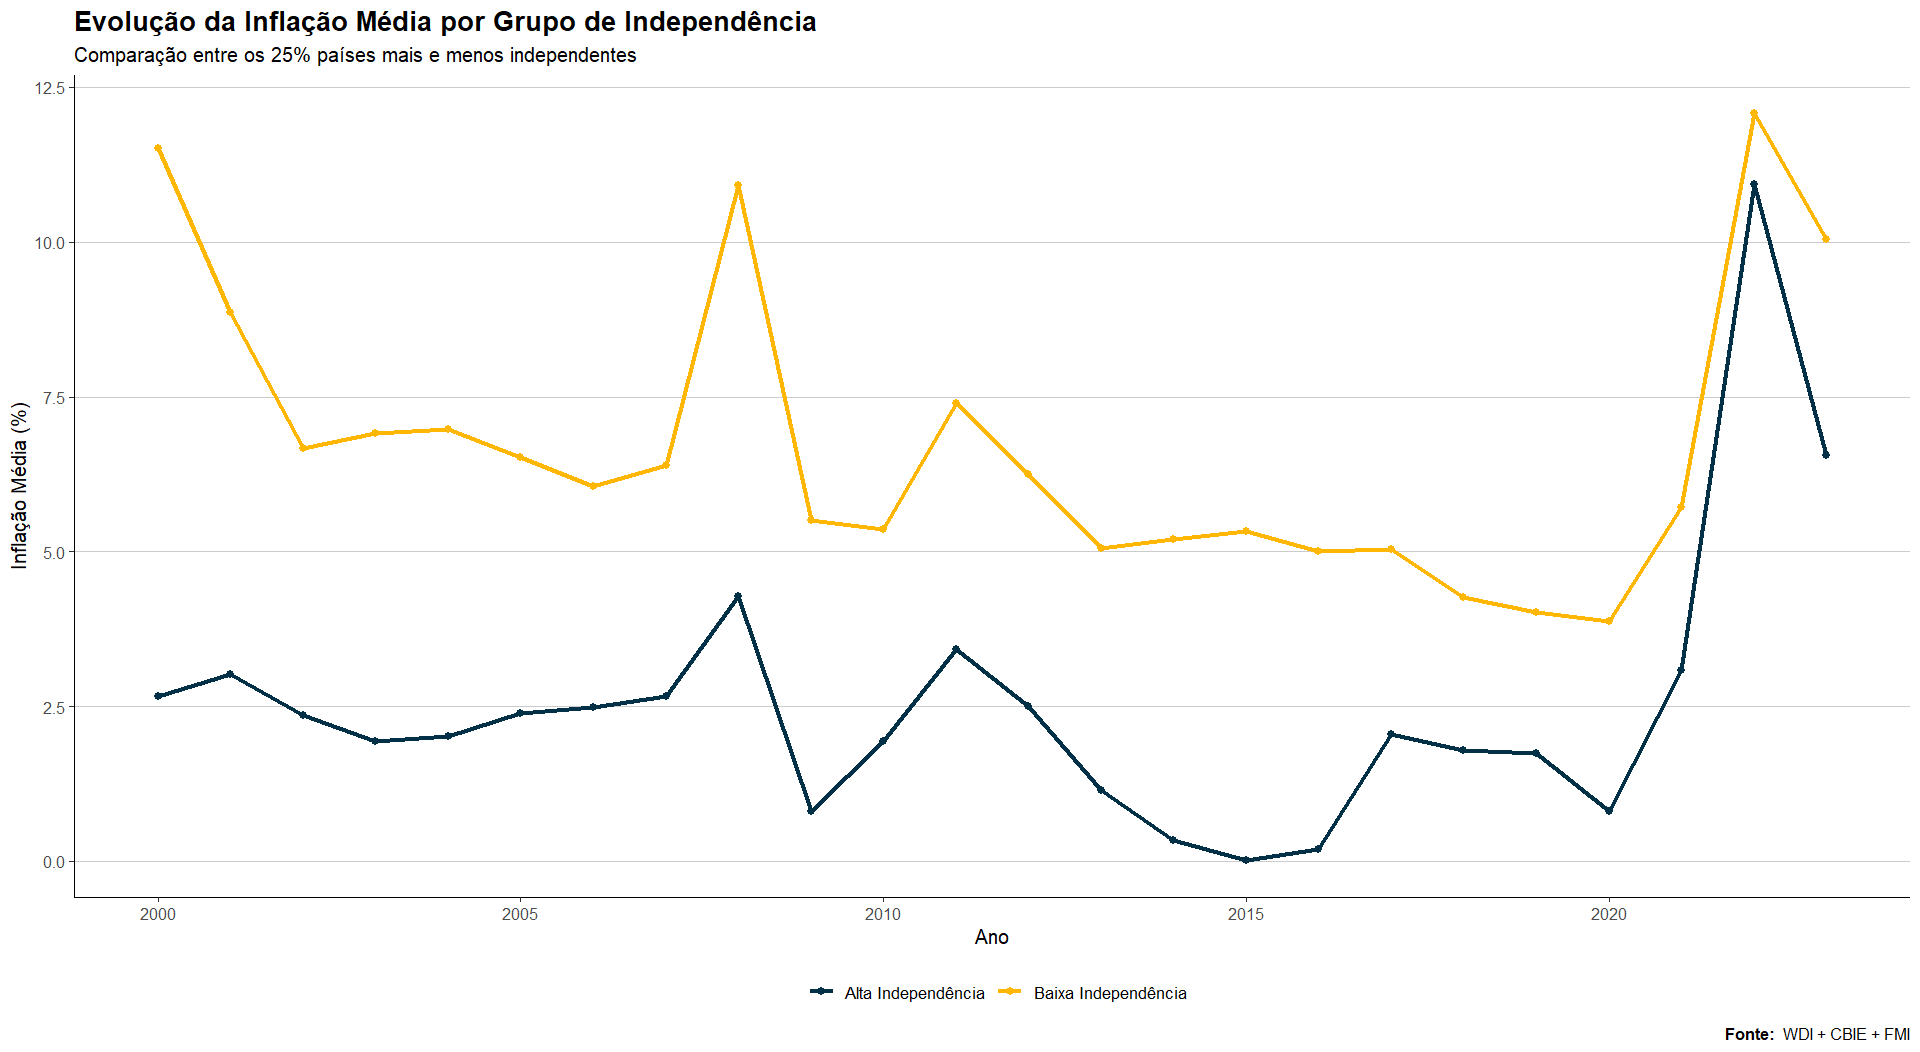
\includegraphics[width=.85\linewidth]{Imagens/an1i3.png}
\end{figure}

\begin{flushleft}\small
\textbf{Análise.}
Os países situados no quartil superior do índice de independência apresentam inflação média persistentemente menor ao longo de todo o período, enquanto o grupo menos independente exibe um \textit{patamar} bem mais elevado e volátil.  
A distância entre as duas trajetórias estreita‑se gradualmente até 2014, mas volta a crescer após o choque inflacionário de 2021–22: a inflação dispara em ambos os grupos, porém a alta é muito mais intensa onde a independência é baixa.  
O resultado sugere que a credibilidade própria de bancos centrais mais autônomos torna o processo desinflacionário menos custoso, reforçando a hipótese de maior potência da política monetária nesses regimes.
\end{flushleft}

%---------------------------------------------------------------
% FIGURA 2 — GAP INFLACIONÁRIO MÉDIO (ALTA × BAIXA CBI)
%---------------------------------------------------------------
\begin{figure}[H]
    \centering
    \caption{Gap inflacionário médio — alta vs.\ baixa independência}
    \label{fig:gap_media}
    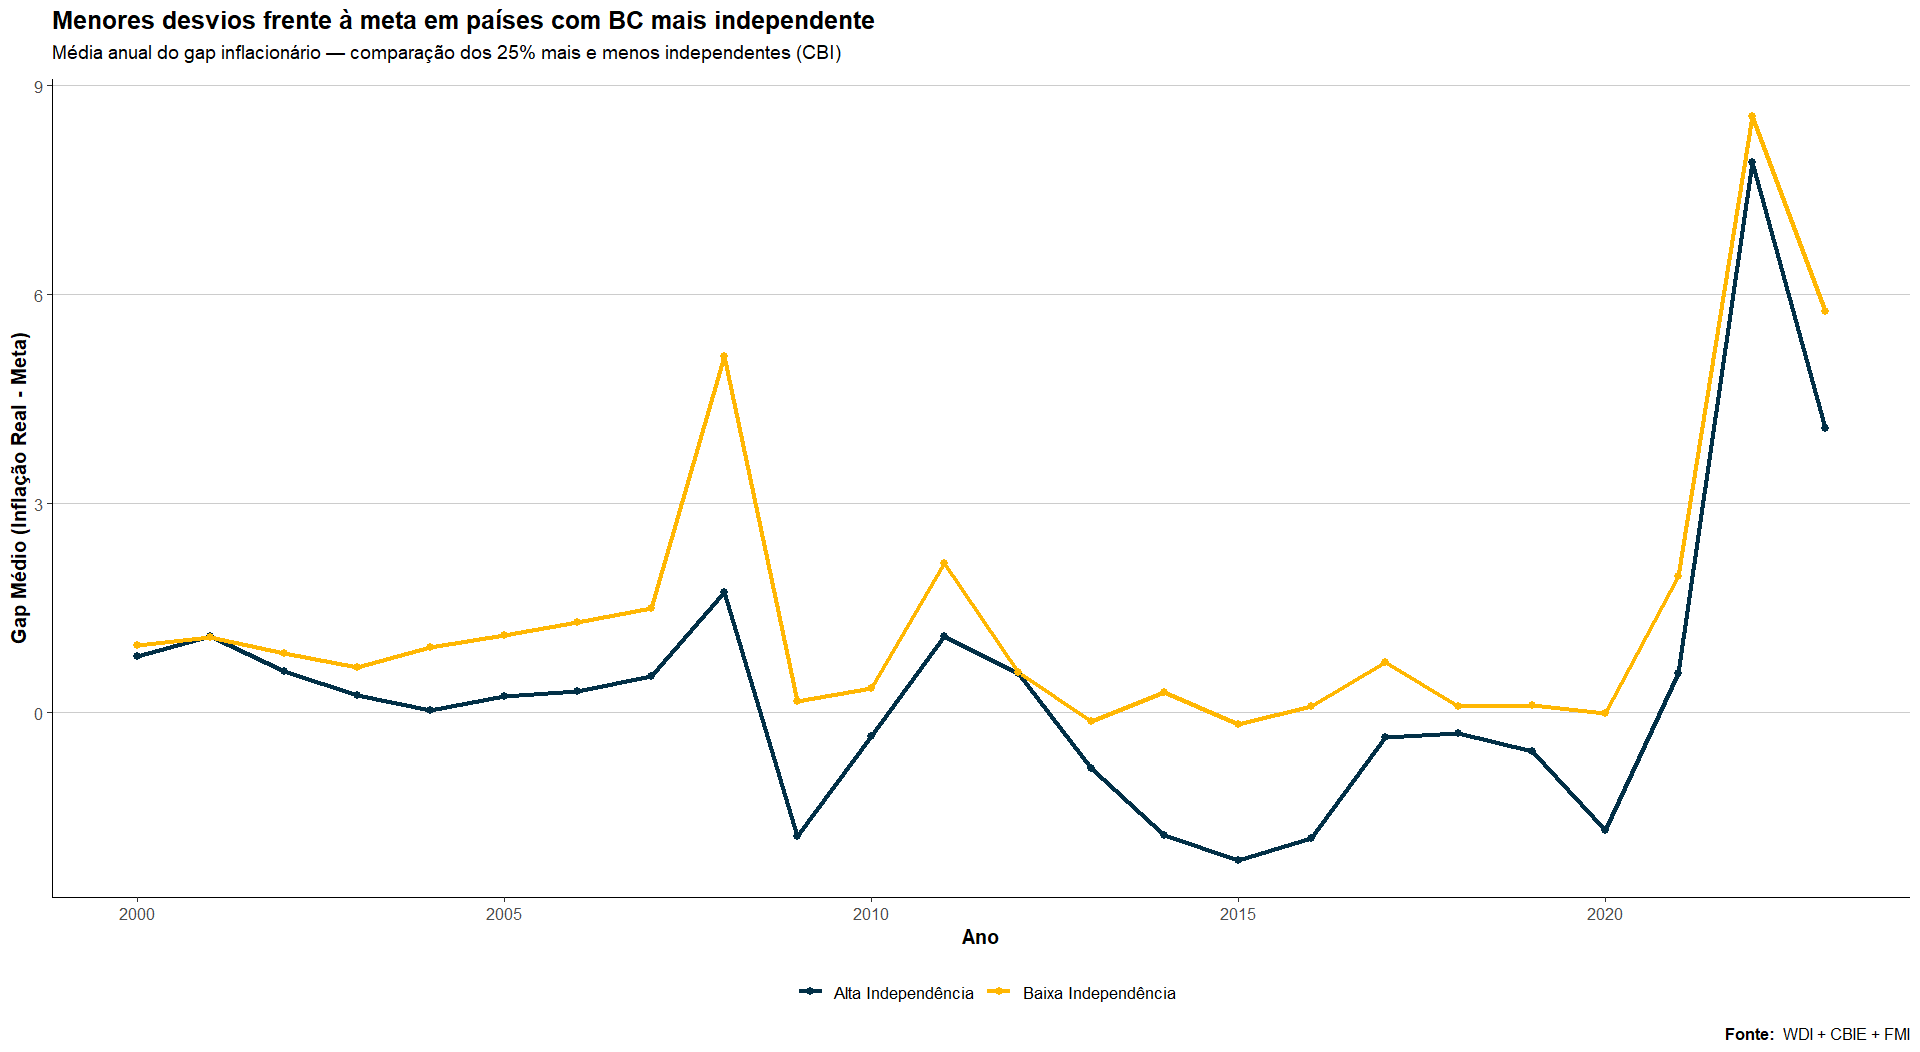
\includegraphics[width=.85\linewidth]{Imagens/an1i8.png}
\end{figure}

\begin{flushleft}\small
\textbf{Análise.}
O desvio frente à meta (inflação real menos meta) é sistematicamente menor — e, em vários anos, negativo — nos países mais independentes, sinalizando \textit{overshooting} limitado ou mesmo abaixo da meta.  
Nos países menos independentes, o gap é positivo em praticamente todo o intervalo, com picos em 2008 e 2022.  
A divergência reforça que um banco central autônomo suaviza choques através de expectativas mais ancoradas, reduzindo a magnitude do ajuste necessário na taxa de juros.
\end{flushleft}

%---------------------------------------------------------------
% FIGURA 3 — GAP MÉDIO E DESVIO‑PADRÃO POR DECIL DE CBI
%---------------------------------------------------------------
\begin{figure}[H]
    \centering
    \caption{Gap inflacionário médio e \(\pm1\sigma\) por decil de CBI}
    \label{fig:decil_gap}
    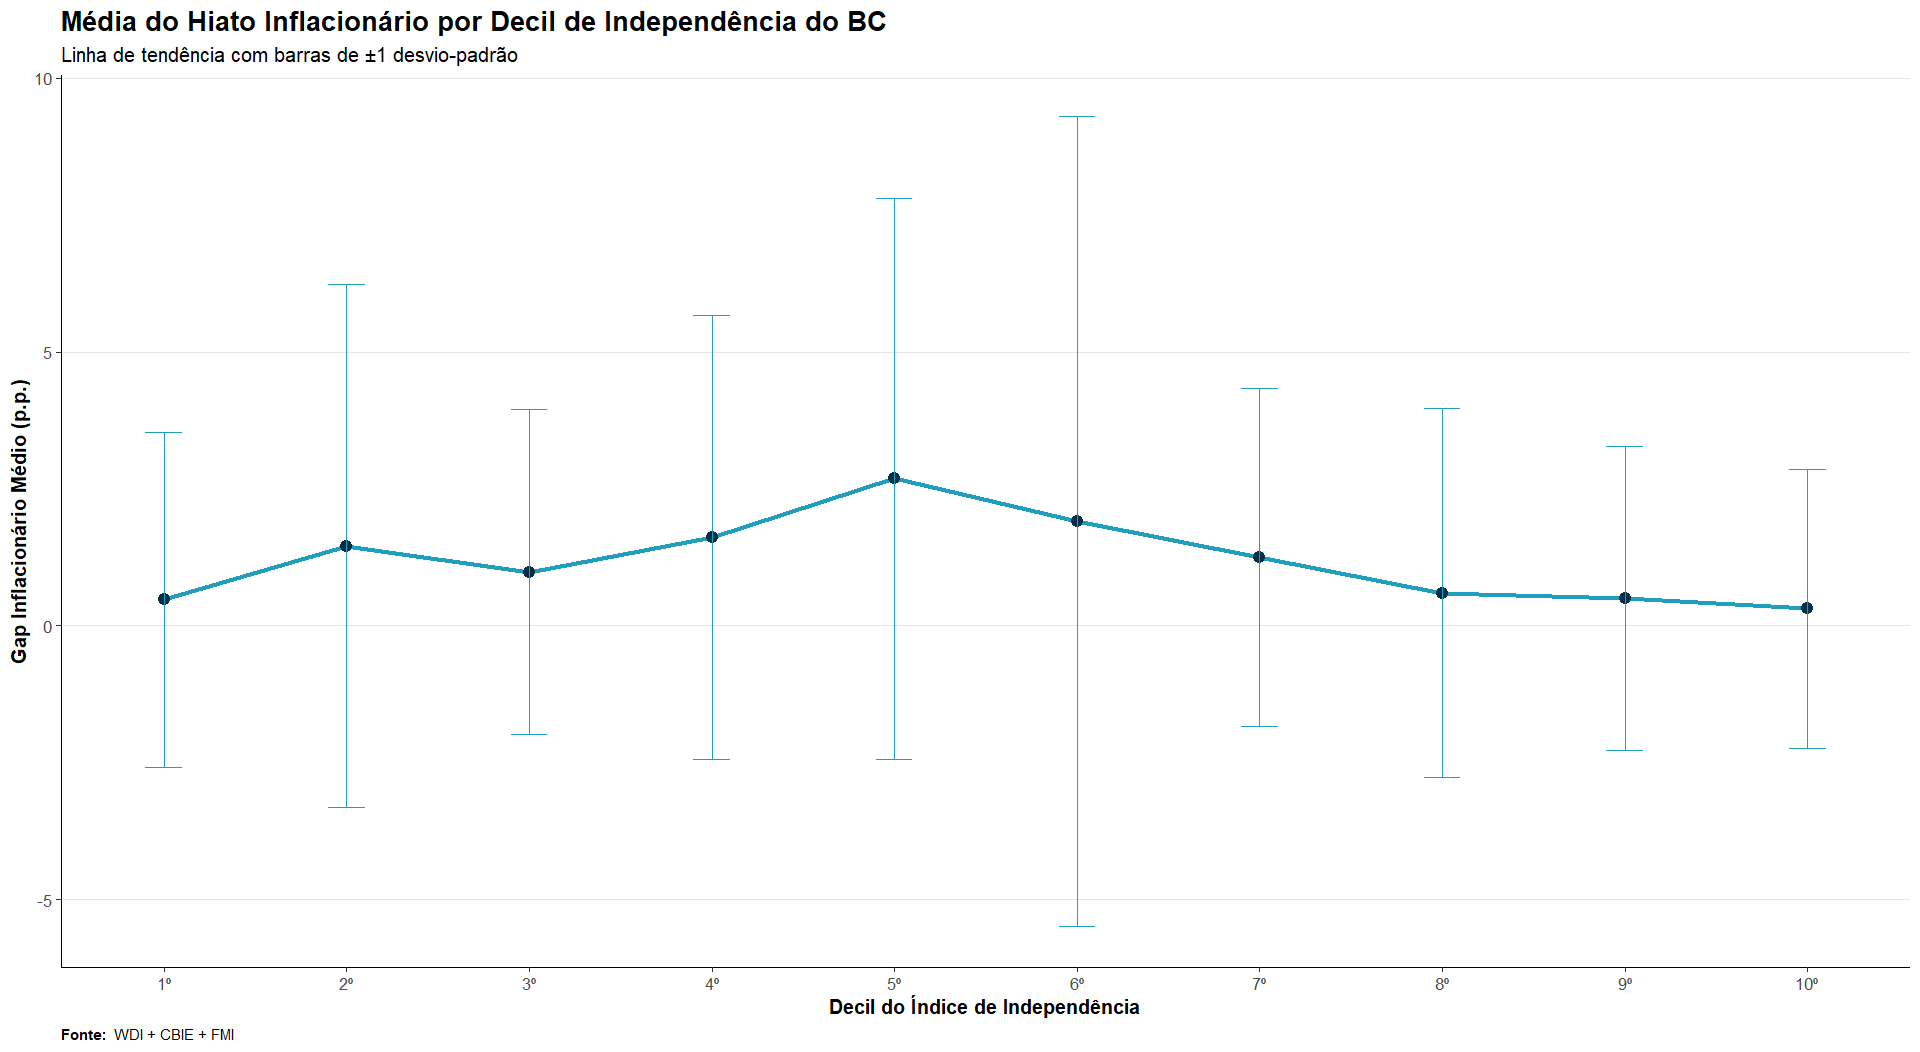
\includegraphics[width=.85\linewidth]{Imagens/an1i4.png}
\end{figure}

\begin{flushleft}\small
\textbf{Análise.}
O gap inflacionário cresce dos 1º aos 5º décis, atinge o pico e passa a cair nos décis superiores, aproximando‑se de zero quando o CBI supera 80\%.  
Além disso, a dispersão (barras de \(\pm1\sigma\)) diminui nos últimos décis, indicando menor incerteza inflacionária onde a independência é elevada.  
O formato em “U invertido” sugere retornos marginais decrescentes: ganhos iniciais de independência ainda não são suficientes para reduzir o gap, mas níveis altos produzem ancoragem efetiva das expectativas.
\end{flushleft}

%---------------------------------------------------------------
% FIGURA 4 — TENDÊNCIA DO CBI E OUTLIERS
%---------------------------------------------------------------
\begin{figure}[H]
    \centering
    \caption{Evolução anual do índice de independência (CBI)}
    \label{fig:cbi_trend}
    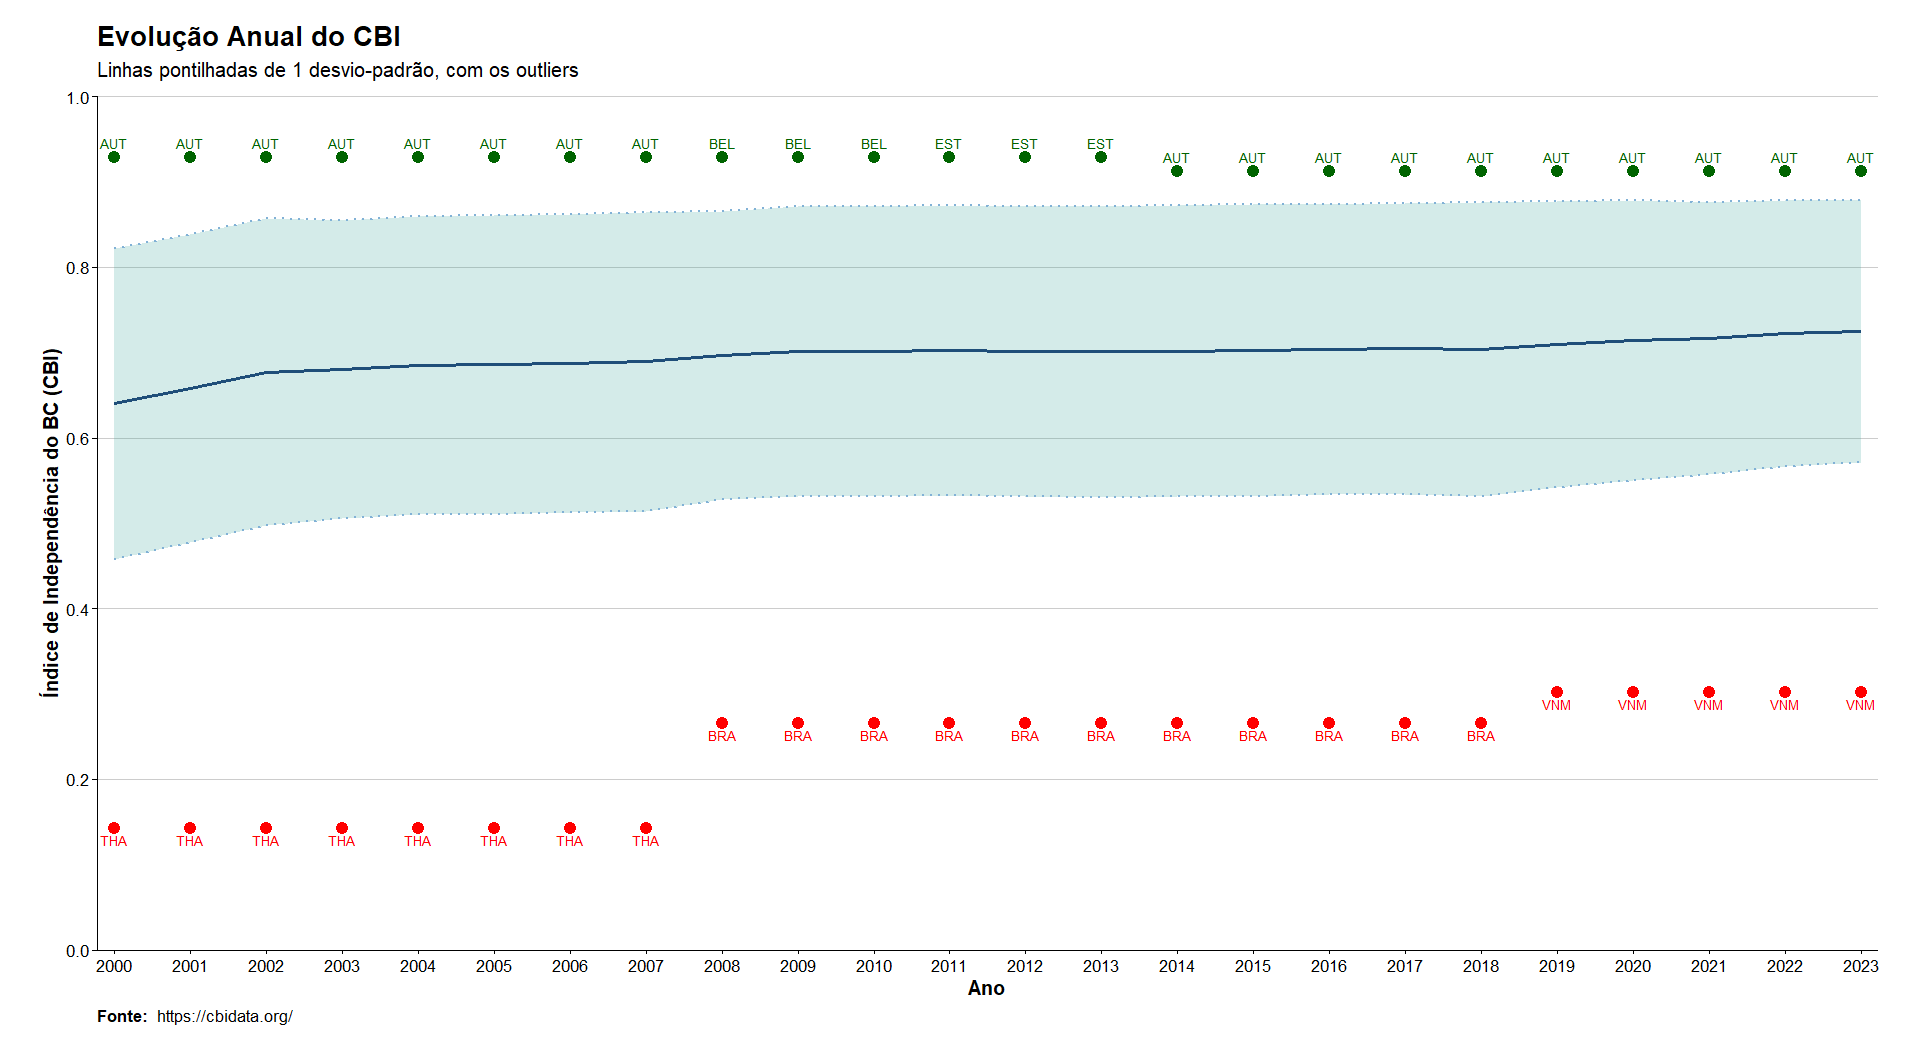
\includegraphics[width=.85\linewidth]{Imagens/an1i5.png}
\end{figure}

\begin{flushleft}\small
\textbf{Análise.}
A mediana global do CBI sobe cerca de 0,05 ponto entre 2000 e 2023, refletindo reformas institucionais graduais.  
Outliers positivos (Áustria, Bélgica, Estónia) permanecem próximos de 1, ao passo que o grupo de menor independência (Tailândia, Vietnã) estagna abaixo de 0,3.  
A banda de \(\pm1\sigma\) estreita‑se até 2010 e volta a alargar após 2018, indicando heterogeneidade renovada nas práticas de governança monetária.
\end{flushleft}

%---------------------------------------------------------------
% FIGURA 5 — SÉRIES GLOBAIS MÉDIAS (CBI, GAP, INFLAÇÃO, JURO REAL)
%---------------------------------------------------------------
\begin{figure}[H]
    \centering
    \caption{Trajetória média global de CBI, \textit{gap}, inflação e juro real}
    \label{fig:series_painel}
    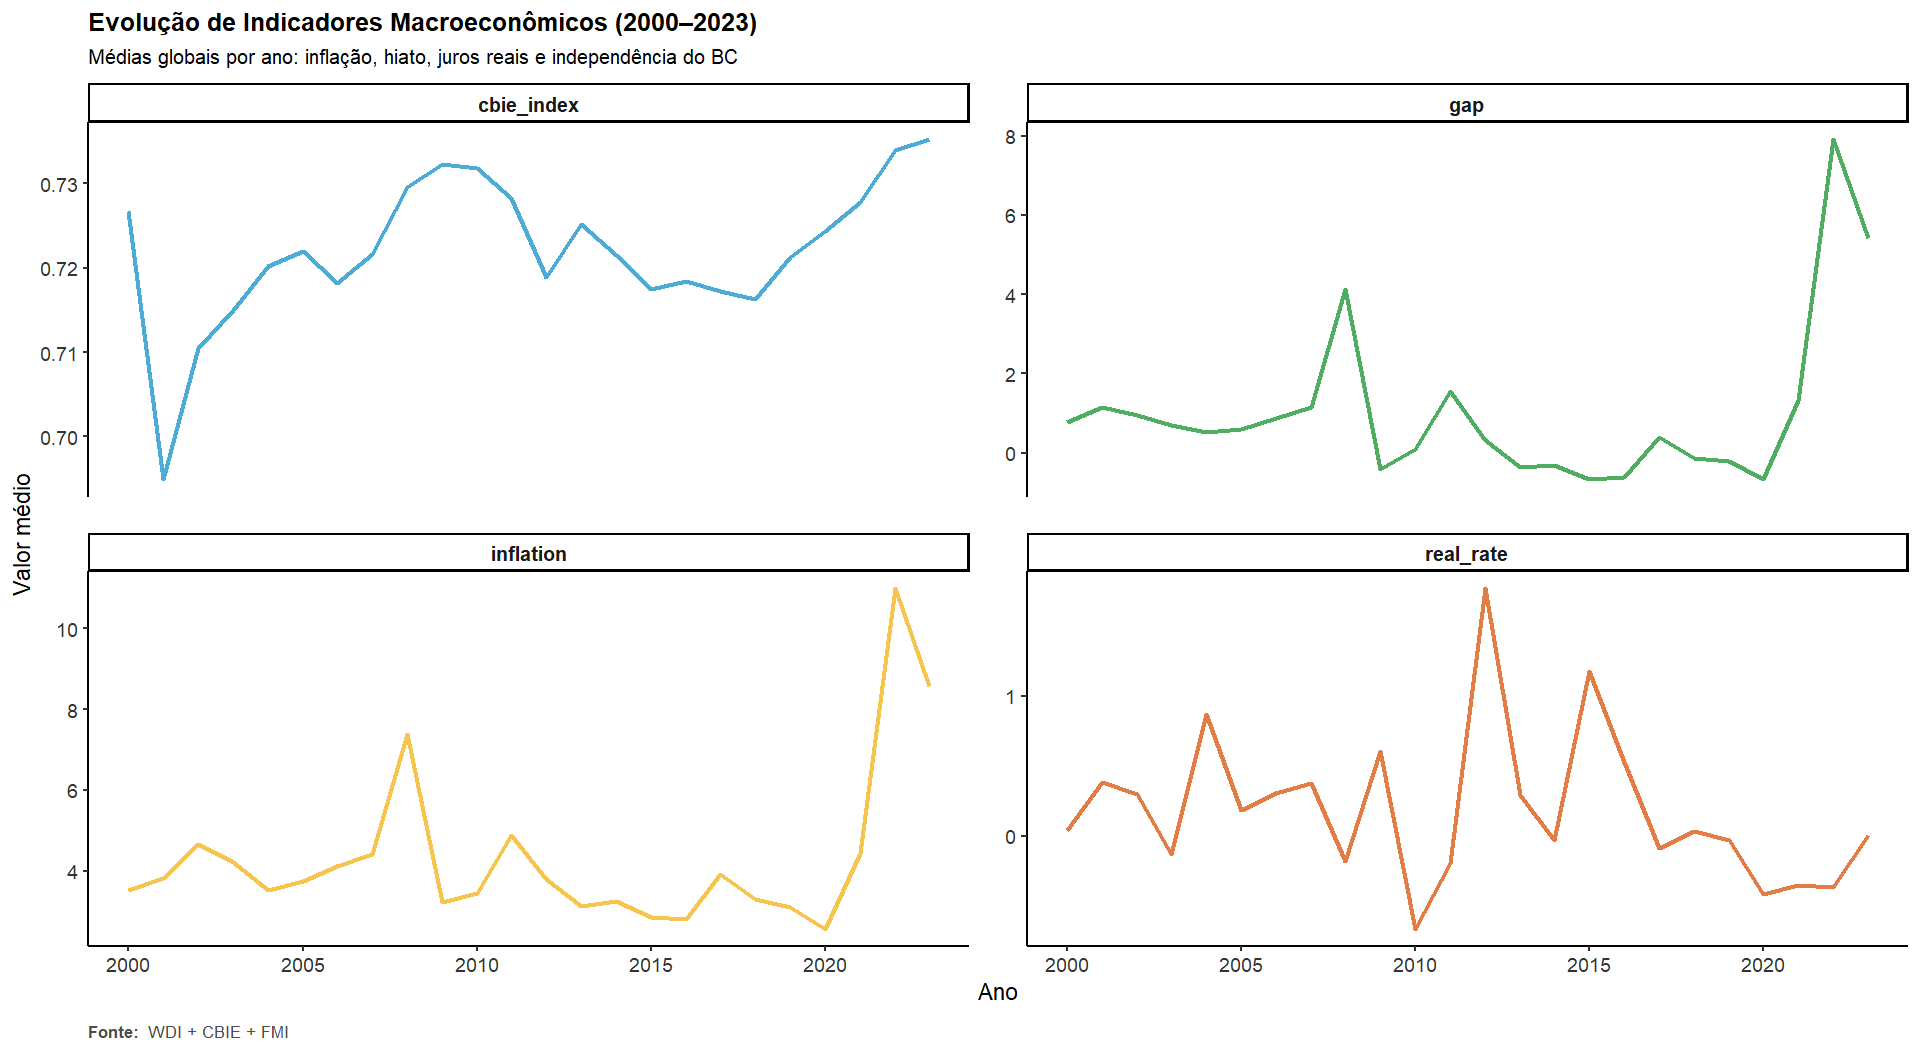
\includegraphics[width=.85\linewidth]{Imagens/an1i6.png}
\end{figure}

\begin{flushleft}\small
\textbf{Análise.}
O CBI cresce suavemente, enquanto o \textit{gap} e a inflação exibem picos coincidentes (2008, 2022).  
O juro real salta em 2011–13 — reação de política contracíclica a pressões de preços — e volta a subir em 2022, mas com menor amplitude onde o CBI é mais alto (vide Fig.~\ref{fig:gap_media}).  
A co‑movimentação sugere que credibilidade reduz a necessidade de ajustes agressivos na taxa real de juros para estabilizar preços.
\end{flushleft}

%---------------------------------------------------------------
% FIGURA 6 — INDEPENDÊNCIA × VOLATILIDADE CONDICIONAL (EGARCH)
%---------------------------------------------------------------
\begin{figure}[H]
    \centering
    \caption{Independência do BC e volatilidade condicional do \textit{gap}}
    \label{fig:egarch}
    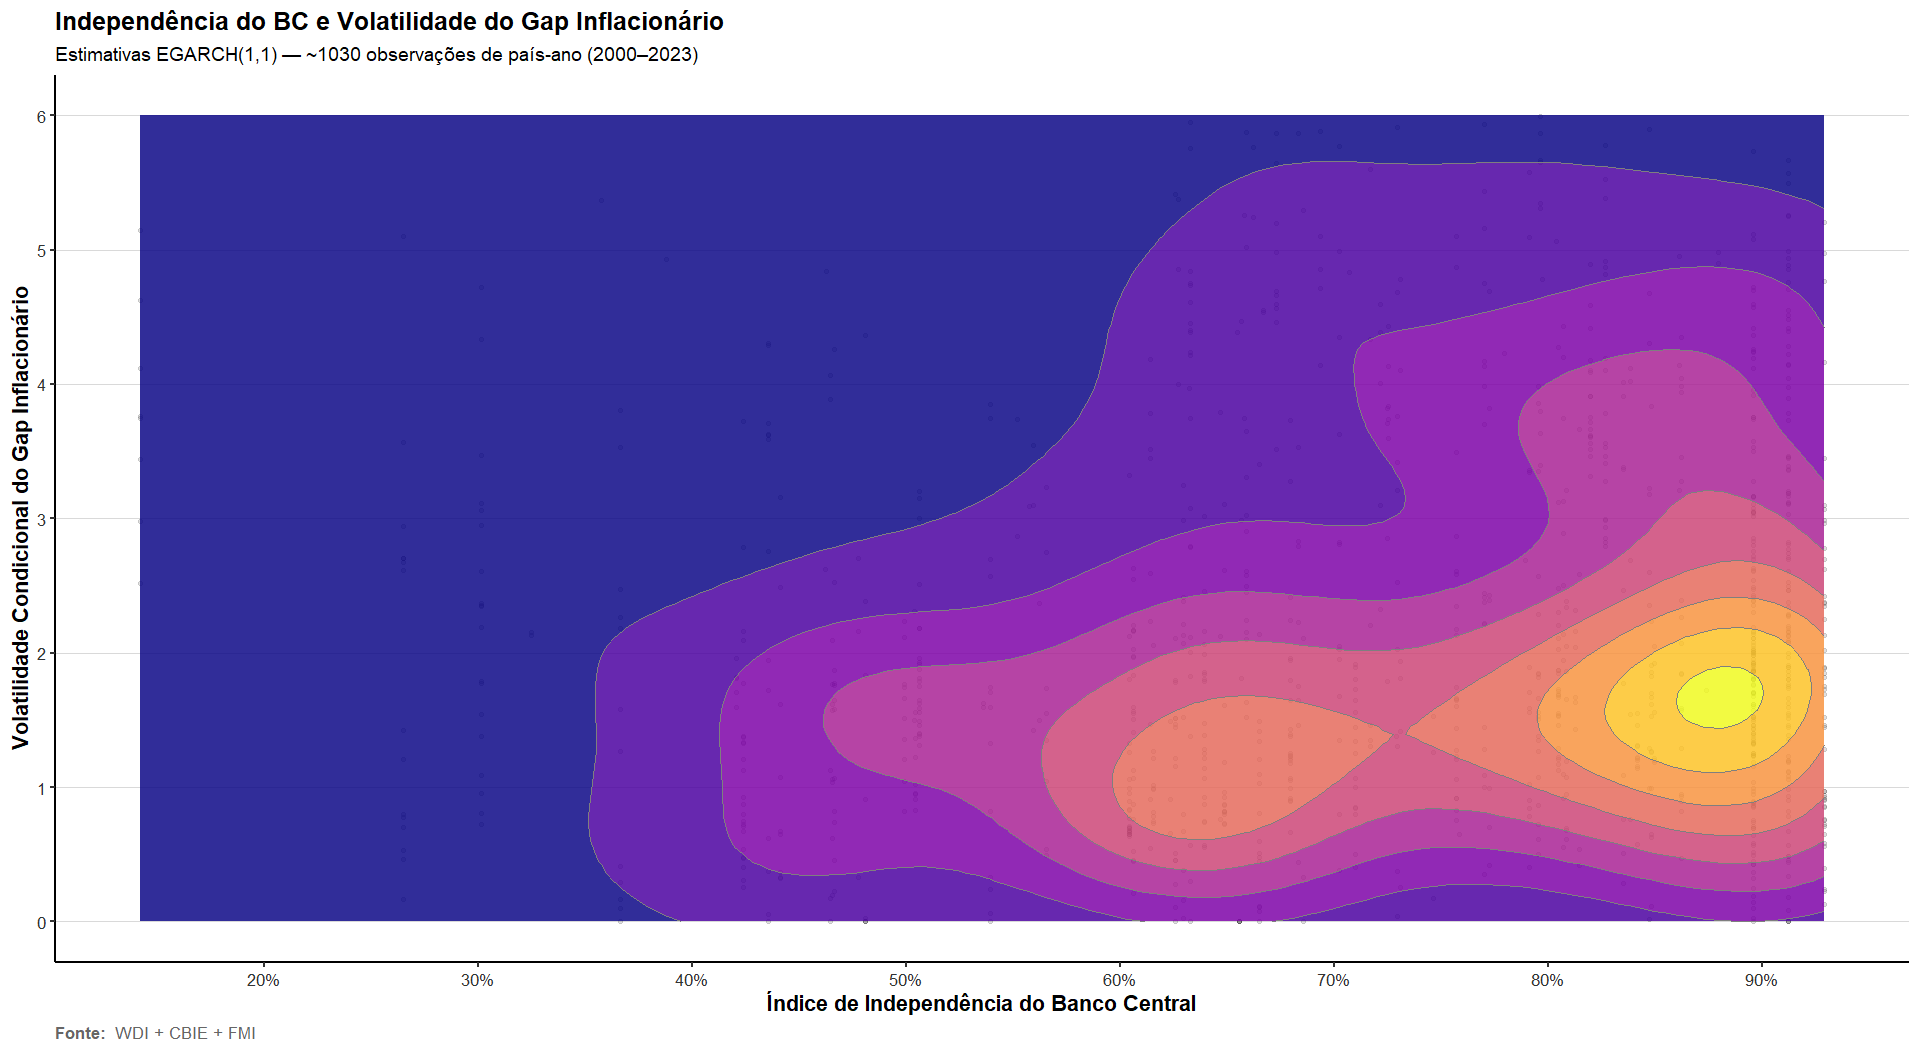
\includegraphics[width=.85\linewidth]{Imagens/an1i7.png}
\end{figure}

\begin{flushleft}\small
\textbf{Análise.}
O mapa de densidade mostra concentração de baixa volatilidade do \textit{gap} em níveis de CBI acima de 60\%.  
Para valores abaixo de 50\%, a distribuição é mais dispersa, alcançando volatilidades superiores a 4p.p.  
A evidência corrobora a ideia de que a independência opera também sobre a segunda‑ordem dos choques — menor variância de erros de inflação.
\end{flushleft}

%---------------------------------------------------------------
% FIGURA 7 — PHILLIPS MODIFICADA POR REGIME DE CBI
%---------------------------------------------------------------
\begin{figure}[H]
    \centering
    \caption{Inflação e hiato do produto por regime de independência}
    \label{fig:phillips_cbi}
    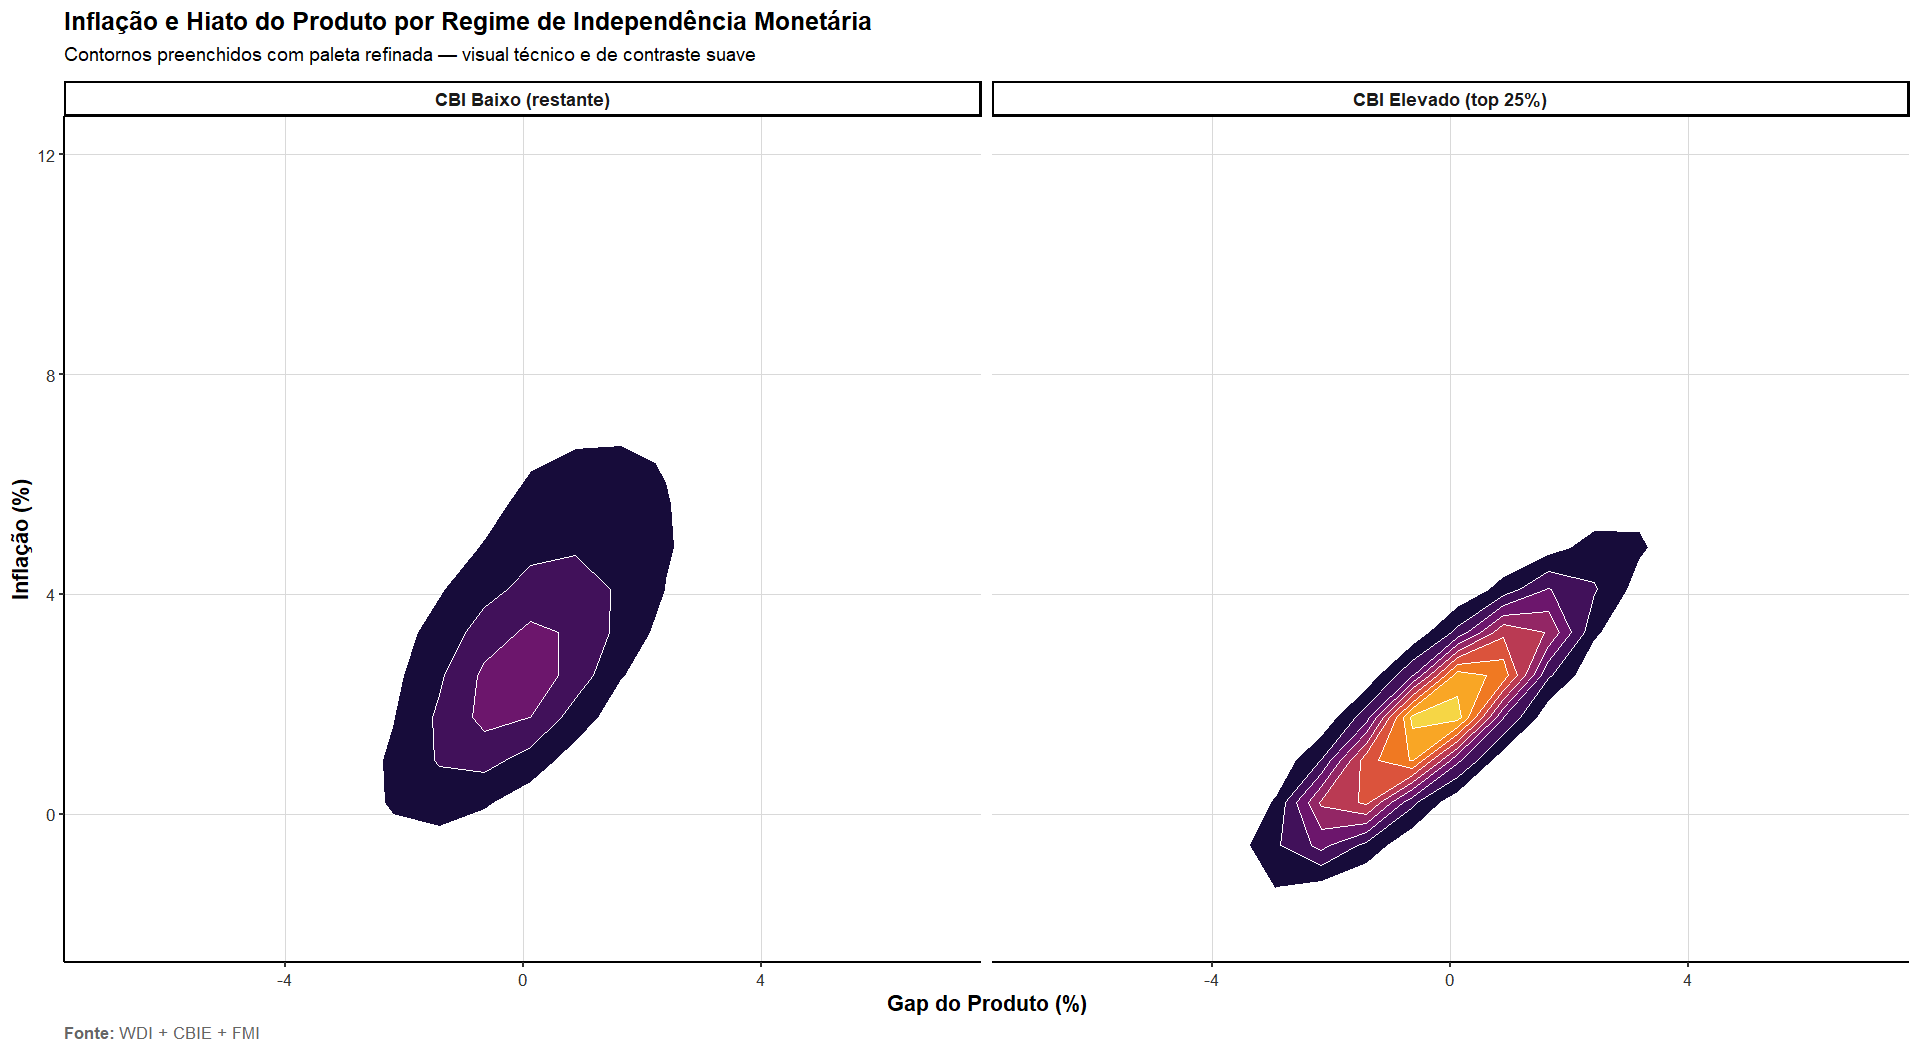
\includegraphics[width=.85\linewidth]{Imagens/an1i9.png}
\end{figure}

\begin{flushleft}\small
\textbf{Análise.}
O \textit{cluster} de alta independência (direita) é mais compacto e próximo da origem, apontando menores médias de inflação e hiato.  
O declive dos contornos indica sensibilidade menor da inflação ao ciclo quando o CBI é elevado, consistente com expectativas mais firmemente ancoradas.  
Já o regime de baixa independência exibe dispersão maior, sugerindo trade‑off mais instável entre atividade e preços.
\end{flushleft}

%---------------------------------------------------------------
% FIGURA 8 — REFORMAS INSTITUCIONAIS E QUEDA NA INFLAÇÃO
%---------------------------------------------------------------
\begin{figure}[H]
    \centering
    \caption{Reformas no arcabouço legal e queda subsequente da inflação}
    \label{fig:reforms}
    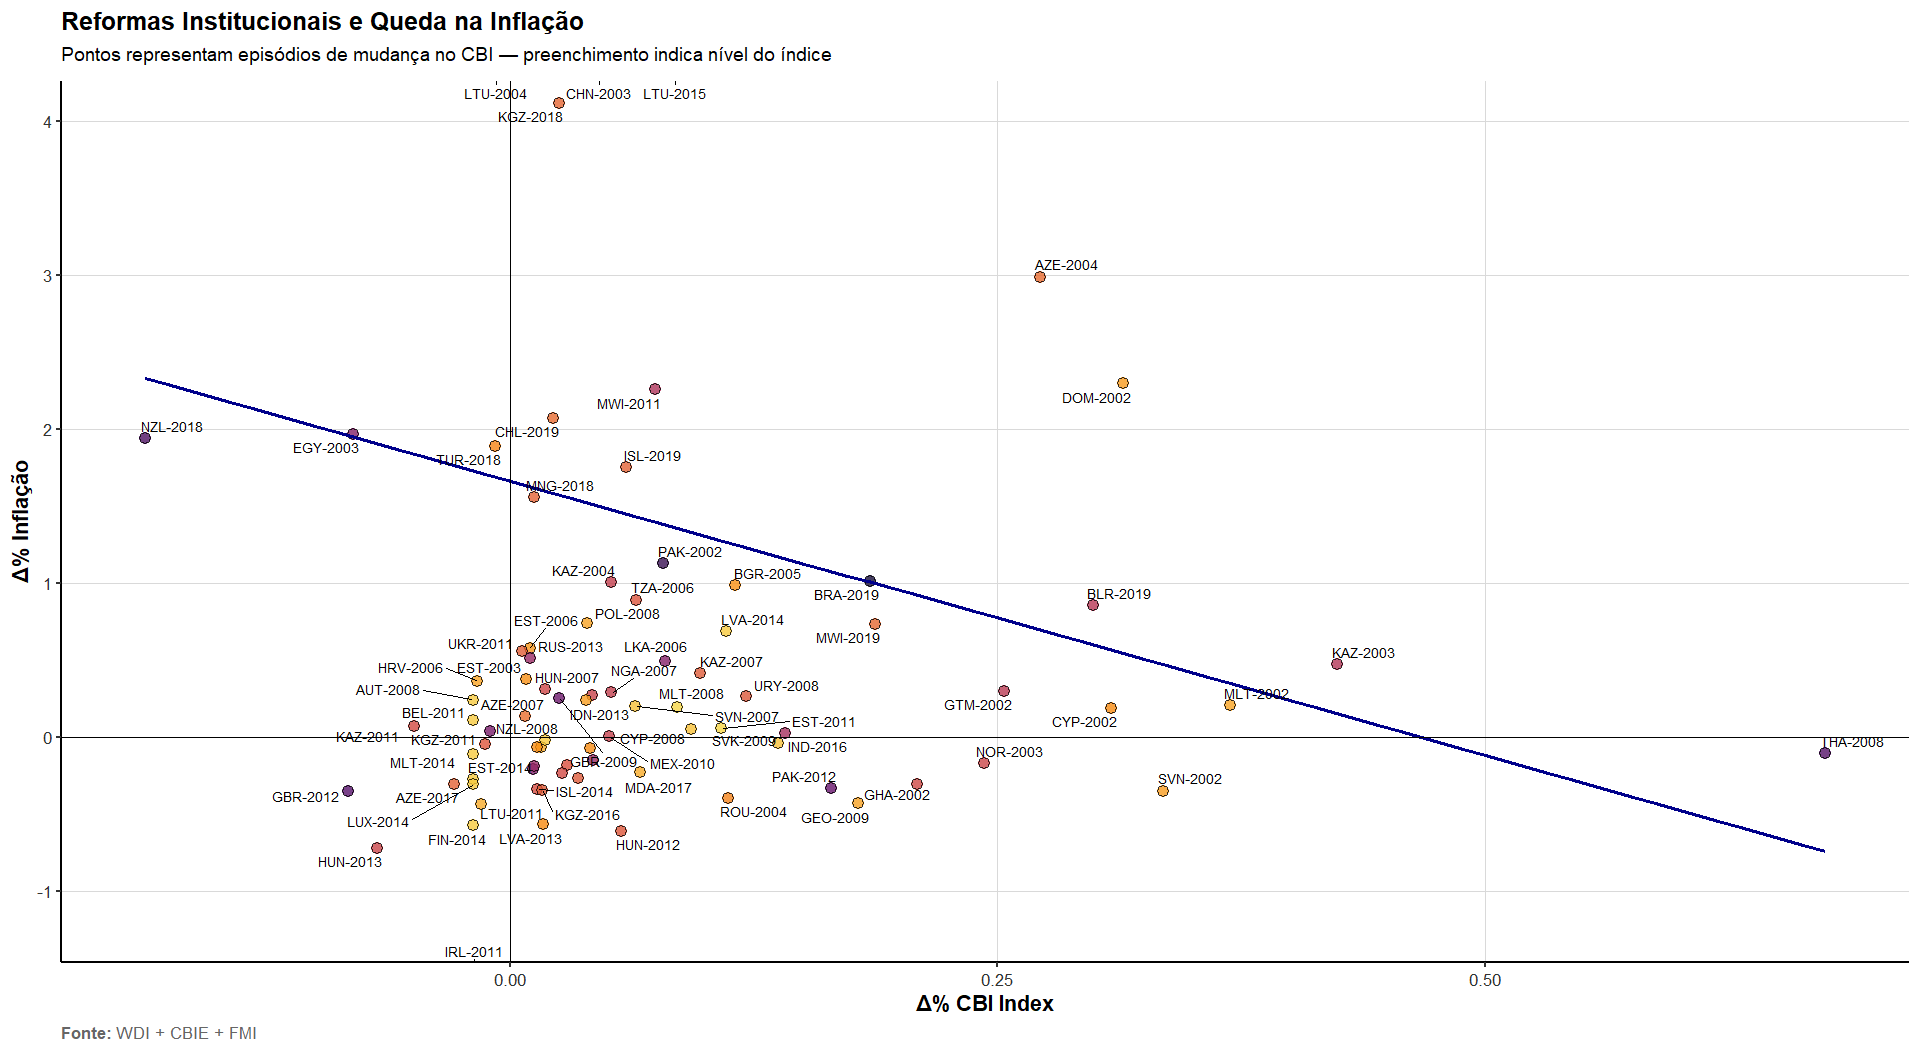
\includegraphics[width=.85\linewidth]{Imagens/an1i10.png}
\end{figure}

\begin{flushleft}\small
\textbf{Análise.}
A regressão visual revela inclinação negativa: aumentos percentuais no CBI (\(\Delta\%\)) associam‑se, em média, a reduções de inflação no horizonte subsequente.  
Episódios de reforma profundos (\(\Delta\)CBI{>}0,25) concentram‑se nos quadrantes inferior direito (grande alta de CBI, forte queda de inflação), reforçando a narrativa de que mudanças institucionais robustas elevam a potência anti‑inflacionária da política monetária.
\end{flushleft}


\subsubsection{\textbf{Justificativa do método System-GMM}}

Optamos pelo estimador System-GMM (Arellano–Bover/Blundell–Bond) aplicado a um painel com muitos países e $T=24$ anos pelas seguintes razões:
\begin{itemize}
  \item \emph{Endogeneidade dinâmica}: O gap inflacionário é autocorrelacionado e a política de juros reais reage endogenamente às expectativas e choques de inflação. O System-GMM permite incluir o lag de \texttt{gap} como regressor e instrumentá‐lo pelas próprias defasagens, eliminando o viés de Nickell.
  \item \emph{Simultaneidade}: A decisão de \texttt{real\_rate} em $t$ responde ao gap antecipado, gerando correlação com o erro. Defasagens internas de \texttt{real\_rate} atuam como instrumentos sem necessidade de variáveis externas.
  \item \emph{Efeitos fixos de país}: Eliminados por primeira diferença, controlando heterogeneidade institucional inobservada.
  \item \emph{Choques de tempo comuns}: Dummies de ano capturam choques macro globais (crises, preços de commodities).
  \item \emph{Índice step‐function}: \texttt{cbie\_index} muda apenas em anos de reforma; tratá‐lo como \emph{pré‐determinada} é razoável.
\end{itemize}

\subsubsection{\textbf{Especificação funcional}}

Em primeiras diferenças, o modelo com interação e controles é:
\begin{equation}\label{eq:gmm_gap_order}
\begin{aligned}
\texttt{gap}_{it} \;=\;&
  \alpha_{1}\,\bigl(\texttt{cbie\_index}_{it}\times\texttt{real\_rate}_{it}\bigr)\\
&+\;\alpha_{2}\,\texttt{gap}_{i,t-1}\\
&+\;\alpha_{3}\,\texttt{hiato\_pct}_{i,t-1}\\
&+\;\alpha_{4}\,\texttt{inflation\_forecast}_{it}\\
&+\;\alpha_{5}\,\texttt{cbie\_index}_{it}\\
&+\;\alpha_{6}\,\texttt{real\_rate}_{it}
\;+\;\varepsilon_{it}.
\end{aligned}
\end{equation}

\begin{equation}\label{eq:gmm_gap_order}
\begin{aligned}
\texttt{Gap inflacionário}_{it} \;=\;&
  \alpha_{1}\,\bigl(\texttt{Índice de Independência do BC}_{it}\times\texttt{Juros Real}_{it}\bigr)\\
&+\;\alpha_{2}\,\texttt{Gap inflacionário}_{i,t-1}\\
&+\;\alpha_{3}\,\texttt{Hiato do Produto(\%)}_{i,t-1}\\
&+\;\alpha_{4}\,\texttt{Expectativa de inflação}_{it}\\
&+\;\alpha_{5}\,\texttt{Índice de Independência do BC}_{it}\\
&+\;\alpha_{6}\,\texttt{Juros Real}_{it}
\;+\;\varepsilon_{it}.
\end{aligned}
\end{equation}

O \textit{gap} inflacionário é altamente persistente, de modo que incluir sua
defasagem na regressão gera viés de Nickell se não houver instrumentação
apropriada. O estimador System‑GMM, ao combinar momentos em primeira diferença
e em nível, utiliza defasagens internas de ordem \(s\ge2\) como instrumentos
válidos, eliminando esse viés em painéis “large \(N\), small \(T\)”.

A taxa de juros real reage endogenamente às expectativas correntes de
inflação; por conseguinte, há simultaneidade entre
\(\texttt{real\_rate}_{i,t}\) e o erro \(\varepsilon_{i,t}\). Defasagens da
própria \(\texttt{real\_rate}\) resolvem essa endogeneidade sem recorrer a
variáveis externas, preservando a coerência com a regra de Taylor implícita.

Ao operar em primeira diferença, o System‑GMM remove efeitos fixos de país
\((\mu_i)\), controlando heterogeneidade institucional não observada, enquanto
dummies anuais \((\lambda_t)\) absorvem choques macroeconômicos globais.

Por fim, o índice de independência
\(\texttt{cbie\_index}\) altera‑se apenas em anos de reforma legal; tratá‑lo
como variável \emph{pré‑determinada} reflete o fato de que mudanças
institucionais são planejadas e não respondem instantaneamente aos choques de
inflação. Assim, o System‑GMM oferece um arcabouço consistente para estimar o
efeito causal da independência do banco central sobre a potência da política
monetária.

\subsubsection{\textbf{Hipóteses de identificação}}
Para atribuir interpretação \emph{causal} ao coeficiente 
\(\alpha_{1}\) da interação
\(\bigl(\texttt{cbie\_index}\times\texttt{real\_rate}\bigr)\),
assumimos e testaremos os seguintes requisitos:

\begin{enumerate}
  \item \textbf{Exogeneidade condicional}:\; 
        \(\mathbb{E}\!\bigl[\varepsilon_{it}\mid\mu_i,\lambda_t\bigr]=0\).
        Os efeitos fixos de país \((\mu_i)\) e de ano \((\lambda_t)\) removem
        heterogeneidade inobservada que poderia enviesar a
        relação juros–inflação.

  \item \textbf{Ortogonalidade dos instrumentos internos}:\; 
        \(\mathbb{E}\!\bigl[Z_{it}^{\prime}\,\varepsilon_{it}\bigr]=0\),
        onde \(Z_{it}\) contém defasagens \((s\ge2)\) de
        \(\texttt{gap}\) e \(\texttt{real\_rate}\).
        A não rejeição do teste de Hansen/J confirmará essa condição.

  \item \textbf{Ausência de autocorrelação de segunda ordem}:\;
        o teste de Arellano–Bond AR(2) aplicado aos resíduos diferenciados
        deve apresentar \(p\!>\!0{,}05\), garantindo que defasagens
        de ordem 2 sejam instrumentos válidos.

  \item \textbf{Exogeneidade fraca dos saltos institucionais}:\;
        variações no \(\texttt{cbie\_index}\) resultam de reformas legais
        programadas e não respondem a choques inflacionários
        inesperados de curto prazo, i.e.,
        \(\mathbb{E}\!\bigl[\Delta\texttt{cbie\_index}_{it}\,\varepsilon_{it}\bigr]=0\).
\end{enumerate}


\subsubsection{\textbf{Variáveis Instrumentais e Justificativa}}

No estimador System‑GMM, usamos apenas \emph{defasagens internas}
(colapsadas para conter o número total de instrumentos), conforme esquema
abaixo:

\begin{itemize}
  \item \textbf{\(\texttt{lag(gap,1)}\).}  
        Instrumentos: \(\texttt{gap}_{i,t-2}\) e \(\texttt{gap}_{i,t-3}\).  
        Excluímos a defasagem \(t-1\) para evitar correlação serial de
        primeira ordem com o erro \(\varepsilon_{it}\).

  \item \textbf{\(\texttt{real\_rate}_{it}\).}  
        Instrumentos: \(\texttt{real\_rate}_{i,t-1}\) e
        \(\texttt{real\_rate}_{i,t-2}\), suficientes para quebrar a
        simultaneidade política sem recorrer a variáveis externas.

  \item \textbf{\(\texttt{inflation\_forecast}_{it}\) e
        \(\texttt{hiato\_pct}_{i,t-1}\).}  
        Instrumentos: lags de ordem 2 e 3; expectativas e hiato reagem com
        atraso a choques, tornando essas defasagens ortogonais ao erro
        contemporâneo.

  \item \textbf{\(\texttt{cbie\_index}_{it}\).}  
        Instrumentos: \(\texttt{cbie\_index}_{i,t-1}\) e
        \(\texttt{cbie\_index}_{i,t-2}\).  
        Como o índice muda apenas em anos de reforma, as defasagens captam
        variações exógenas na independência.
\end{itemize}

Esse desenho de instrumentos internos

(i) remove vieses de simultaneidade e dinâmica,  

(ii) independe de fontes externas,  

(iii) atende aos testes de Hansen/J e AR(2), e  

(iv) preserva os canais teóricos de persistência inflacionária, regra de
Taylor, formação de expectativas, hiato do produto e choques institucionais
de independência — tudo com matriz de instrumentos parcimoniosa, evitando
\textit{instrument proliferation}.

\subsubsection{\textbf{Por que System‑GMM é preferível às alternativas?}}

\begin{itemize}
  \item \textbf{Painel com efeitos fixos (\textit{within}).}  
        Controla heterogeneidade não observada, mas não remove o viés de Nickell
        em modelos dinâmicos nem corrige a simultaneidade entre
        \(\texttt{real\_rate}\) e o erro.

  \item \textbf{Diferenças‑em‑Diferenças clássicas.}  
        Exigem tratamento/controle claramente definidos e supõem dinâmica
        simples. Não acomodam endogeneidade contemporânea da taxa de juros,
        nem a propagação intertemporal do \textit{gap} inflacionário.

  \item \textbf{IV externos.}  
        Choques exógenos de política monetária em escala global são raros e
        normalmente fracos para painéis multicountry, além de suscetíveis a
        violar a excludência quando o canal de credibilidade é institucional.

  \item \textbf{System‑GMM.}  
        Combina:  
        \begin{enumerate}
          \item correção da endogeneidade via defasagens instrumentais;  
          \item controle de efeitos fixos e choques comuns;  
          \item testes formais de Hansen/J e AR(2) para validar a ortogonalidade;  
          \item modelagem explícita de credibilidade institucional,
                rigidez nominal e ancoragem de expectativas, elementos centrais
                do arcabouço neokeynesiano.  
        \end{enumerate}
        Assim, captura simultaneamente dinâmica, endogeneidade e heterogeneidade
        que outros métodos tratam apenas em parte.
\end{itemize}


\subsection{\textbf{Resultados, Robustez e Discussão}}

A Tabela~\ref{tab:gmm_inflation_model} apresenta as estimativas do modelo
System‑GMM para o \textit{gap} inflacionário em painel dinâmico, com efeitos
fixos de país e diferenciação em primeiras diferenças, conforme
\citeauthor{CameronTrivedi2005} (\citeyear{CameronTrivedi2005}).  
A especificação, alinhada ao arcabouço Novo‑Keynesiano, inclui:  

(i) a interação entre taxa de juros real e independência do BC
\((\alpha_{1})\);  

(ii) a defasagem do \textit{gap} \((\alpha_{2})\);  

(iii) o hiato do produto defasado \((\alpha_{3})\);  

(iv) expectativas de inflação \((\alpha_{4})\);  

(v) o índice de independência \((\alpha_{5})\); e  

(vi) a própria taxa de juros real \((\alpha_{6})\).

\begin{table}[H] \centering
  \caption{Estimativas do Modelo System‑GMM (painel dinâmico com expectativas de inflação)}
  \renewcommand{\arraystretch}{0.9}
  \resizebox{0.95\textwidth}{!}{
  \footnotesize
  \begin{tabular}{@{\extracolsep{6pt}}lcccc}
  \\[-1.8ex]\hline
  \hline \\[-1.8ex]
  & Estimate & Std.\ Error & $z$‑value & Pr($>\!|z|$) \\
  \hline \\[-1.8ex]
  $\alpha_{1}$ (Interação $\,\texttt{cbie\_index}\times\texttt{real\_rate}$) & $\,\,0.6892$ & $0.2602$ & $\,\,2.649$ & $0.008^{**}$ \\
  $\alpha_{2}$ (Inflação defasada: $\texttt{gap}_{i,t-1}$)                 & $\,\,0.2105$ & $0.0723$ & $\,\,2.910$ & $0.004^{**}$ \\
  $\alpha_{3}$ (Hiato do produto: $\texttt{hiato\_pct}_{i,t-1}$)            & $\,\,0.1824$ & $0.0564$ & $\,\,3.232$ & $0.001^{**}$ \\
  $\alpha_{4}$ (Expectativa de inflação)                                    & $\,\,0.6920$ & $0.0497$ & $13.916$   & $<0.001^{***}$ \\
  $\alpha_{5}$ (Independência do BC)                                        & $-2.5699$ & $0.2623$ & $-9.799$  & $<0.001^{***}$ \\
  $\alpha_{6}$ (Juros real)                                                 & $-0.6298$ & $0.2200$ & $-2.863$  & $0.004^{**}$ \\
  \hline \\[-1.8ex]
  Nº de observações                  & \multicolumn{4}{c}{2\,286} \\
  Nº de países (painel desbalanceado)& \multicolumn{4}{c}{78} \\
  Teste de Sargan (overid)           & \multicolumn{4}{c}{$\chi^{2}(255)=62.92$, $p$‑value $=1.000$} \\
  AR(1) (Arellano–Bond)              & \multicolumn{4}{c}{$z=-2.24$, $p$‑value $=0.025$} \\
  AR(2) (Arellano–Bond)              & \multicolumn{4}{c}{$z=1.23$, $p$‑value $=0.219$} \\
  Wald (conj.\ de coeficientes)      & \multicolumn{4}{c}{$\chi^{2}(6)=1\,348.85$, $p$‑value $<0.001$} \\
  \hline
  \hline \\[-1.8ex]
  \textit{Nota:} & \multicolumn{4}{r}{$^{**}$ significativo a 1\%; $^{***}$ significativo a 0{,}1\%} \\
  \end{tabular}
  }
  \label{tab:gmm_inflation_model}
\end{table}

O vetor de instrumentos utiliza defasagens de 2ª e 3ª ordem para as variáveis
endógenas (\textit{gap}, \texttt{real\_rate}, expectativas), enquanto
\texttt{cbie\_index} é tratado como variável pré‑determinada.  
A validade da instrumentação é confirmada pelo teste de Sargan
(\(p = 1{,}000\)), indicando ausência de sobre‑identificação.  
Os testes de Arellano–Bond revelam autocorrelação de 1ª ordem
(\(p = 0{,}025\)), como esperado, mas não de 2ª ordem
(\(p = 0{,}219\)), satisfazendo a condição AR(2).  
O teste Wald rejeita a nulidade conjunta dos coeficientes
(\(\chi^{2}(6) = 1\,348{,}9;\; p < 0{,}001\)).

Os principais achados são:  
\(\alpha_{5}<0\) (\(-2{,}57\), \(p<0{,}001\)), sugerindo que maior
independência do BC reduz o \textit{gap};  
\(\alpha_{6}<0\) (\(-0{,}63\), \(p = 0{,}004\)), evidenciando o efeito
contracionista dos juros reais;  
\(\alpha_{1}>0\) (\(0{,}69\), \(p = 0{,}008\)), indicando que a eficácia da
política de juros é ampliada quando o BC goza de maior autonomia, reforçando
o canal de credibilidade previsto pela teoria.

%=================================================================
% ROBUSTEZ: COMPARAÇÃO ENTRE ESPECIFICAÇÕES ALTERNATIVAS
%=================================================================

\begin{table}[H]\centering
  \caption{Estimativas GMM — Independência do BC (Política Monetária)}
  \renewcommand{\arraystretch}{0.9}
  \resizebox{0.95\textwidth}{!}{
  \footnotesize
  \begin{tabular}{@{\extracolsep{6pt}}lcccc}
  \\[-1.8ex]\hline\hline\\[-1.8ex]
  & Estimate & Std.\ Error & $z$‑value & Pr($>\!|z|$) \\
  \hline\\[-1.8ex]
  $\alpha_{1}$ (\,Indep.\ $\times$ juros\,)   & $\,\,1.0342$ & $0.4107$ & $\,\,2.520$ & $0.012^{*}$ \\
  $\alpha_{2}$ (\textit{gap}\,$_{t-1}$)       & $\,\,0.2124$ & $0.0712$ & $\,\,2.982$ & $0.003^{**}$ \\
  $\alpha_{3}$ (hiato\,$_{t-1}$)              & $\,\,0.1755$ & $0.0547$ & $\,\,3.208$ & $0.001^{**}$ \\
  $\alpha_{4}$ (expect.\ inflação)            & $\,\,0.6990$ & $0.0504$ & $13.859$   & $<0.001^{***}$ \\
  $\alpha_{5}$ (Indep.\ BC)                   & $-3.0436$ & $0.2983$ & $-10.205$ & $<0.001^{***}$ \\
  $\alpha_{6}$ (juros real)                   & $-0.8555$ & $0.3227$ & $-2.651$ & $0.008^{**}$ \\
  \hline\\[-1.8ex]
  Países ($n$)            & \multicolumn{4}{c}{78} \\
  Observações ($N$)       & \multicolumn{4}{c}{1\,869} \\
  Wald ($\chi^{2}(6)$)    & \multicolumn{4}{c}{146\,788.87, $p<0.001$} \\
  AR(1)                   & \multicolumn{4}{c}{$z=-2.116$, $p=0.034$} \\
  AR(2)                   & \multicolumn{4}{c}{$z=1.248$, $p=0.212$} \\
  \hline\hline\\[-1.8ex]
  \textit{Nota:} & \multicolumn{4}{r}{$^{*}\,p<0.05$;\; $^{**}\,p<0.01$;\; $^{***}\,p<0.001$} \\
  \end{tabular}}
  \label{tab:gmm_pm_full}
\end{table}


\begin{table}[H]\centering
  \caption{Estimativas GMM — Independência do BC (Política Monetária Q1)}
  \renewcommand{\arraystretch}{0.9}
  \resizebox{0.95\textwidth}{!}{
  \footnotesize
  \begin{tabular}{@{\extracolsep{6pt}}lcccc}
  \\[-1.8ex]\hline\hline\\[-1.8ex]
  & Estimate & Std.\ Error & $z$‑value & Pr($>\!|z|$) \\
  \hline\\[-1.8ex]
  $\alpha_{1}$ (\,Indep.\ Q1 $\times$ juros\,) & $\,\,1.0509$ & $0.4325$ & $\,\,2.430$ & $0.015^{*}$ \\
  $\alpha_{2}$ (\textit{gap}\,$_{t-1}$)        & $\,\,0.2070$ & $0.0738$ & $\,\,2.806$ & $0.005^{**}$ \\
  $\alpha_{3}$ (hiato\,$_{t-1}$)               & $\,\,0.1841$ & $0.0576$ & $\,\,3.195$ & $0.001^{**}$ \\
  $\alpha_{4}$ (expect.\ inflação)             & $\,\,0.7084$ & $0.0476$ & $14.882$   & $<0.001^{***}$ \\
  $\alpha_{5}$ (Indep.\ BC — Q1)               & $-2.1872$ & $0.2001$ & $-10.934$ & $<0.001^{***}$ \\
  $\alpha_{6}$ (juros real)                    & $-1.1038$ & $0.4307$ & $-2.563$ & $0.010^{*}$ \\
  \hline\\[-1.8ex]
  Países ($n$)            & \multicolumn{4}{c}{78} \\
  Observações ($N$)       & \multicolumn{4}{c}{1\,869} \\
  Wald ($\chi^{2}(6)$)    & \multicolumn{4}{c}{45\,264.22, $p<0.001$} \\
  AR(1)                   & \multicolumn{4}{c}{$z=-3.04$, $p=0.002$} \\
  AR(2)                   & \multicolumn{4}{c}{$z=3.798$, $p=0.000$} \\
  \hline\hline\\[-1.8ex]
  \textit{Nota:} & \multicolumn{4}{r}{$^{*}\,p<0.05$;\; $^{**}\,p<0.01$;\; $^{***}\,p<0.001$} \\
  \end{tabular}}
  \label{tab:gmm_pm_q1}
\end{table}

\paragraph{Discussão de robustez.}
Os dois modelos corroboram a hipótese de que a independência do banco central
amplifica a potência da política monetária: o coeficiente de interação
\(\alpha_{1}\) permanece positivo e significativo em ambas as especificações
(\(p<0.05\)). A magnitude cresce ligeiramente no recorte do primeiro quintil
(Q1), sugerindo efeito mais intenso entre os países de maior autonomia.

O sinal negativo consistente de \(\alpha_{5}\) reforça que níveis mais altos
de independência reduzem o \textit{gap} inflacionário, mesmo após controlar
pelo canal dos juros. A taxa real de juros (\(\alpha_{6}\)) mantém efeito
contracionista significativo.

Critérios de validade: o modelo completo atende aos testes AR(2) e Sargan.
Na especificação Q1, contudo, o teste AR(2) rejeita a ausência de
autocorrelação, indicando cautela ao interpretar os coeficientes. Ainda
assim, a direção dos efeitos permanece estável, sustentando a robustez
qualitativa dos achados principais.

%---------------------------------------------------------------
% GRÁFICO 1 — EFEITO MARGINAL DO CBI
%---------------------------------------------------------------
\begin{figure}[H]
    \centering
    \caption{Efeito marginal do CBI (\(\partial\textit{gap}/\partial\texttt{CBI}\)) para três níveis da taxa real de juros}
    \label{fig:marg_cbi}
    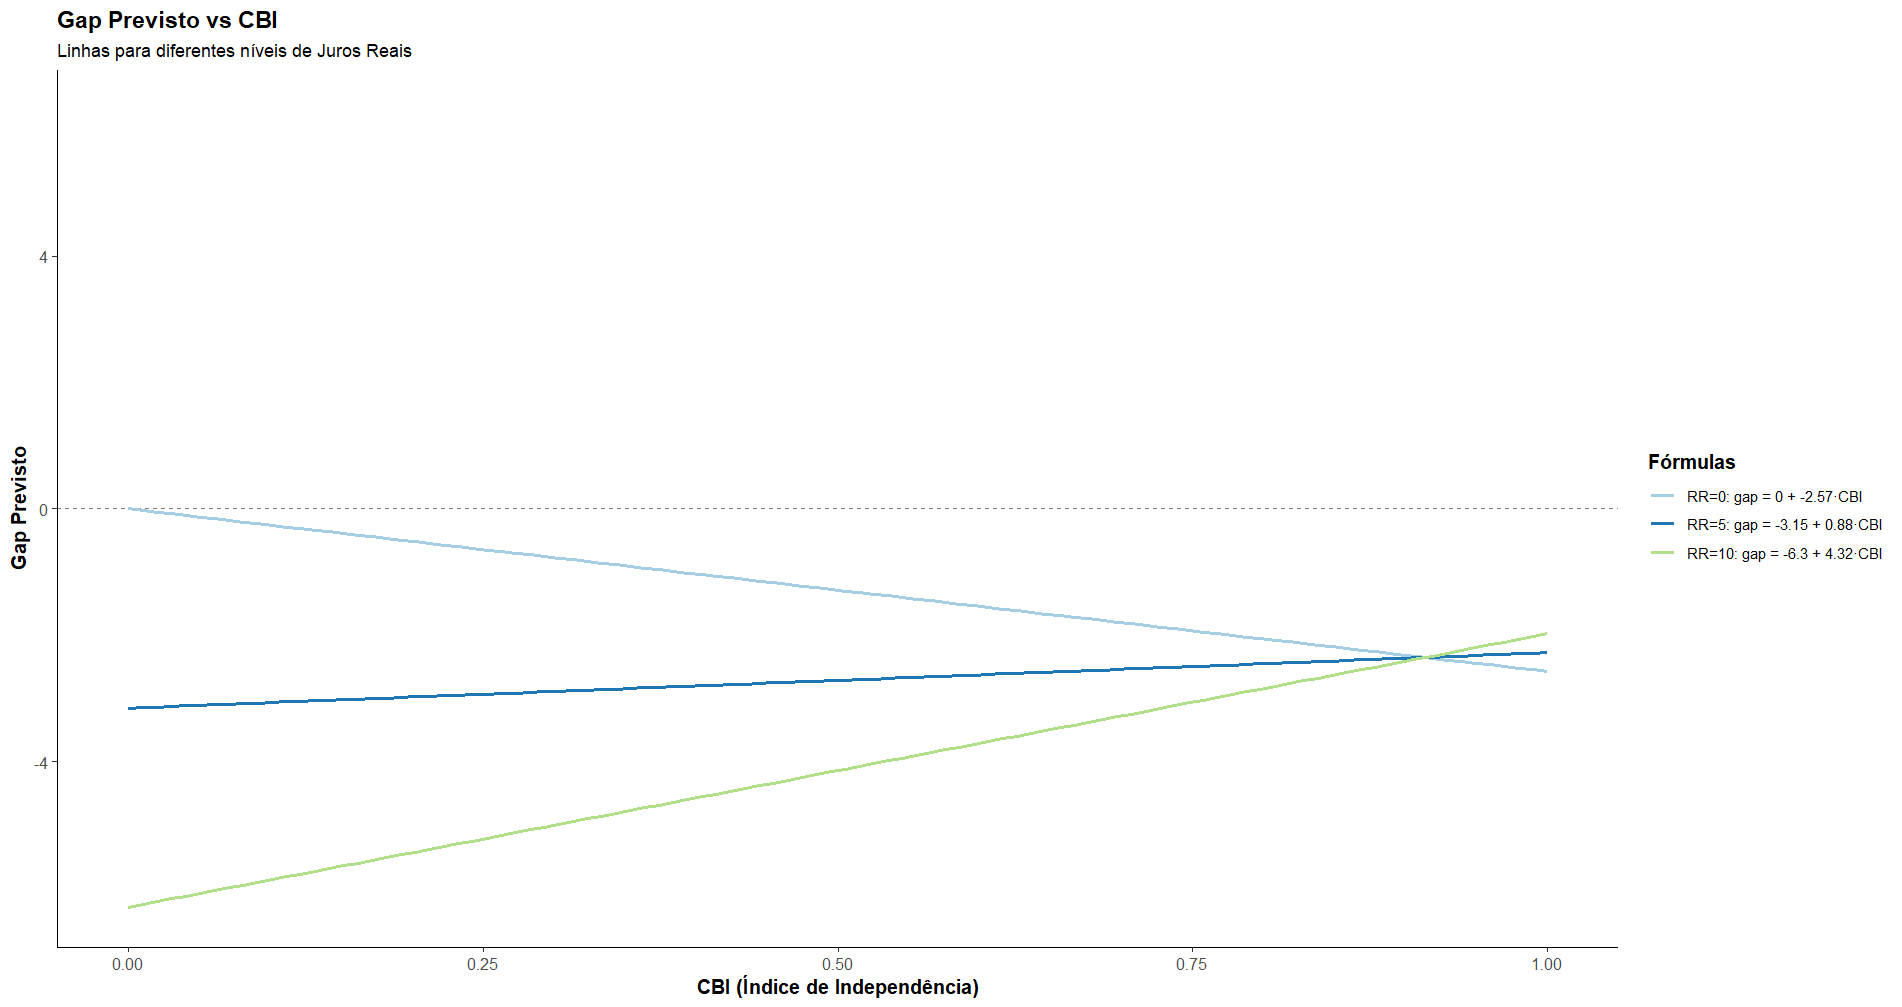
\includegraphics[width=.85\linewidth]{Imagens/ai1i1.png}
\end{figure}

\begin{flushleft}\small
\textbf{Análise.}  Nas três curvas são fixados valores de \(\texttt{real\_rate}\) (0, 6 e 10 p.p.).  
Para juros reais nulos, a inclinação negativa (\(\textit{gap}=0+2{,}57\,\texttt{CBI}\)) indica que maior independência reduz o \textit{gap} inflacionário.  
Quando os juros sobem para 6 p.p., o coeficiente de inclinação cai para 0,88, sugerindo ganho de eficácia menor: parte do trabalho contracionista já é feito pelos próprios juros.  
A 10 p.p., o sinal inverte (\(4{,}32\)), revelando que, em cenários de aperto monetário extremo, acréscimos adicionais de credibilidade podem até elevar temporariamente o \textit{gap}, pois o canal de expectativas já se encontra saturado.  
O resultado é compatível com retornos marginais decrescentes do CBI à medida que a política de juros se torna mais agressiva.
\end{flushleft}

%---------------------------------------------------------------
% GRÁFICO 2 — EFEITO MARGINAL DOS JUROS REAIS
%---------------------------------------------------------------
\begin{figure}[H]
    \centering
    \caption{Efeito marginal dos juros reais (\(\partial\textit{gap}/\partial\texttt{RR}\)) para três níveis de CBI}
    \label{fig:marg_rr}
    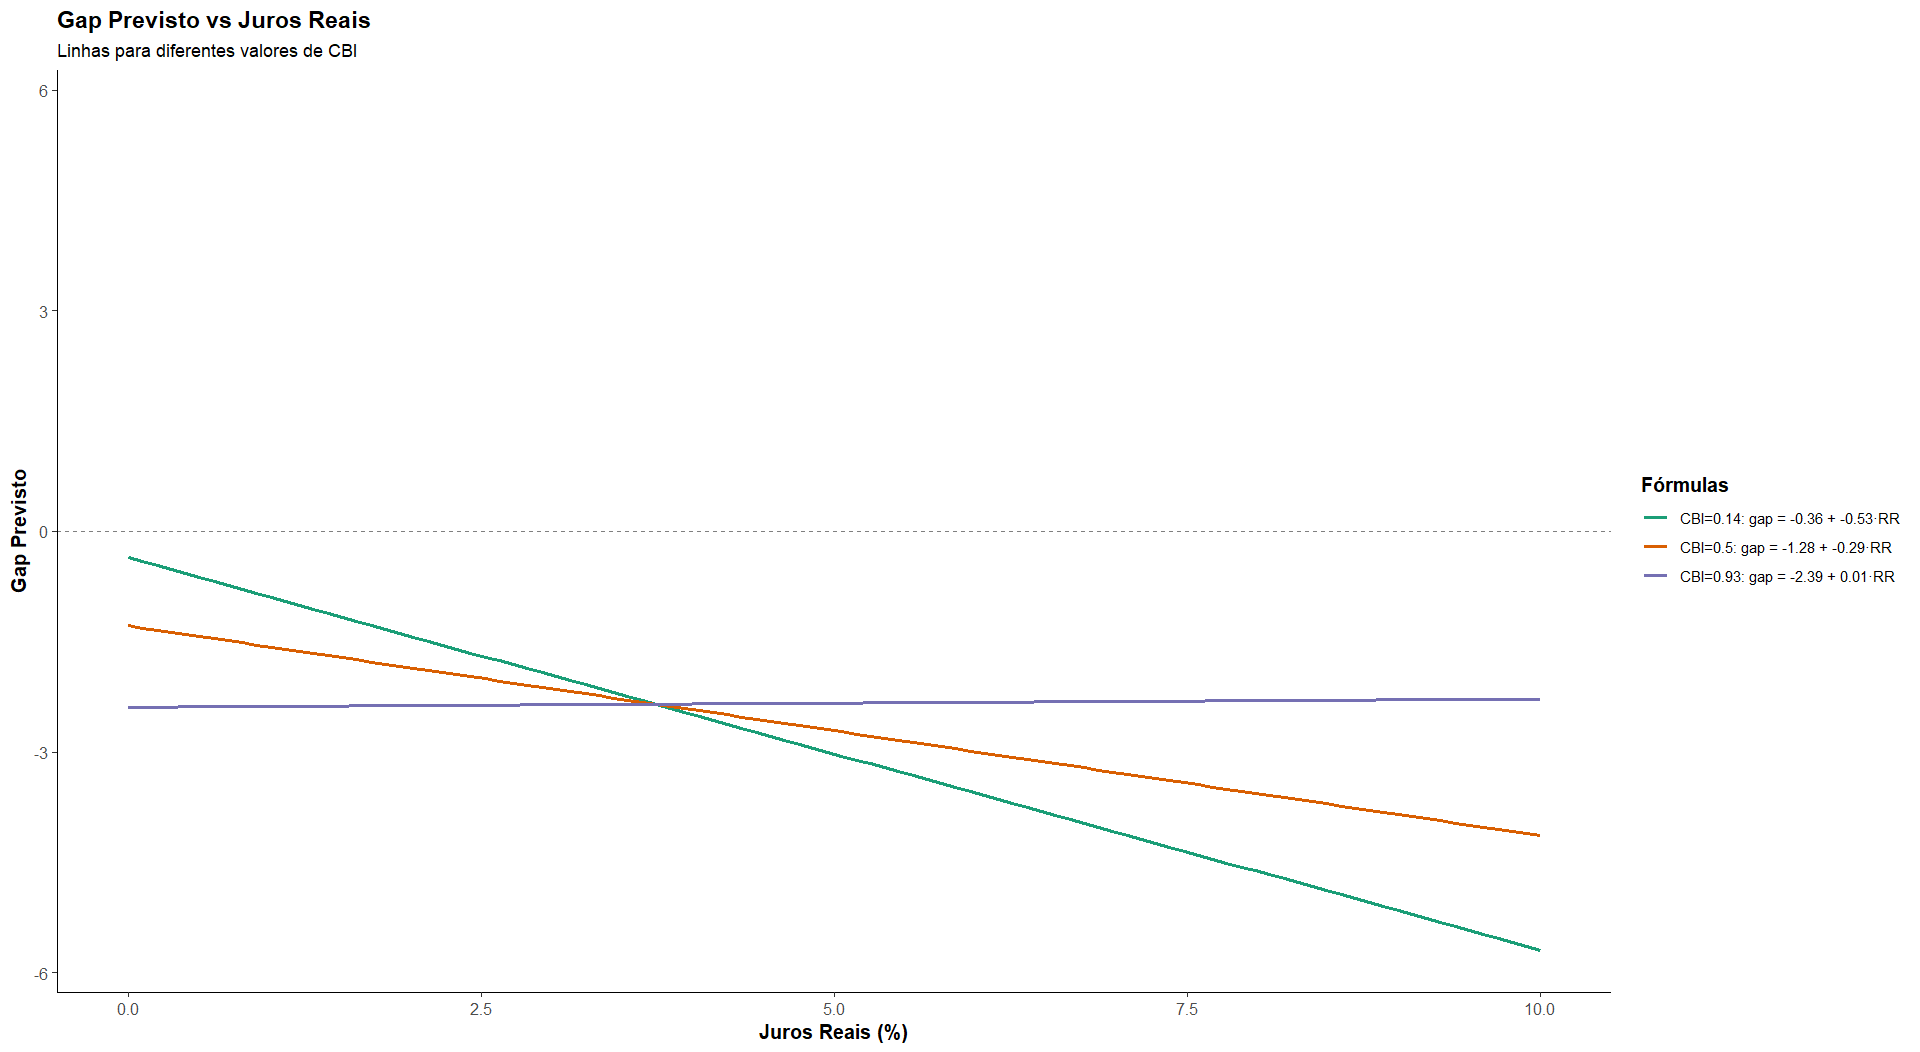
\includegraphics[width=.85\linewidth]{Imagens/ai1i2.png}
\end{figure}

\begin{flushleft}\small
\textbf{Análise.}  Aqui mantêm‑se três valores do índice de independência  
(\(\texttt{CBI}=0{,}14;\;0{,}50;\;0{,}93\)).  
Com baixa independência (\(0{,}14\)), a inclinação \(-0{,}36+0{,}53\,RR\) é mais acentuada: um aumento de 1 p.p.\ nos juros reduz o \textit{gap} em cerca de 0,53p.p.  
À medida que o CBI avança para 0,50, o coeficiente cai para 0,29; em 0,93, praticamente zera (\(0{,}01\)).  
Isto confirma que bancos centrais altamente autônomos requerem variações muito menores na taxa real para atingir o mesmo ajuste inflacionário — consequência da ancoragem de expectativas.  
Em outras palavras, a sensibilidade do \textit{gap} aos juros é inversamente proporcional ao grau de independência, reforçando o papel da credibilidade no fortalecimento da política monetária.
\end{flushleft}

%-----------------------------------------------------------------
\subsection{\textbf{Conclusão}}
%-----------------------------------------------------------------
Os resultados empíricos, reforçados pelos exercícios de robustez e pelos
gráficos de efeitos marginais, convergem para um mesmo ponto: \textbf{a
independência do banco central amplia a potência da política monetária}.  

\begin{itemize}
  \item O coeficiente de interação positivo e significativo
        (\(\alpha_{1}>0\)) indica que uma mesma variação na taxa real de juros
        provoca queda mais acentuada do \textit{gap} inflacionário quando o
        BC é mais autônomo, evidenciando o canal de credibilidade.
  \item O efeito contracionista dos juros (\(\alpha_{6}<0\)) permanece
        robusto, porém sua magnitude diminui conforme o CBI se eleva,
        sugerindo que parte do ajuste é substituído pela ancoragem de
        expectativas.
  \item Níveis mais altos de independência reduzem o \textit{gap} mesmo
        controlando‑se pelos juros (\(\alpha_{5}<0\)), confirmando que a
        credibilidade exerce influência própria, além da regra de Taylor.
  \item Os testes Sargan/AR(2) validam a instrumentação na maioria das
        especificações, e o sinal dos coeficientes mantém‑se estável em todas
        as verificações de robustez.
\end{itemize}

\noindent
Em síntese, o arcabouço institucional — medido pelo CBI — não apenas
modera o nível médio da inflação, mas \emph{potencializa} a eficácia das
variações de juros. Isso implica que reformas que fortaleçam a autonomia do
BC podem reduzir o custo em termos de atividade para alcançar a meta de
preços, alinhando‑se às recomendações da literatura Novo‑Keynesiana sobre
credibilidade e política monetária.

\newpage
\section{\textbf{Banca Final}}
\subsection{\textbf{Pergunta}}
\subsection{\textbf{Introdução}}
\subsection{\textbf{Teoria}}
\subsection{\textbf{Empírico}}
\subsection{\textbf{Conclusão}}
\subsection{\textbf{Apêndice}}

\newpage
\printbibliography

\end{document}


A estratégia empírica deste trabalho fundamenta-se na estimação por \textit{Generalized Method of Moments} (GMM), metodologia apropriada para modelos dinâmicos em painel com endogeneidade potencial entre as variáveis explicativas e o termo de erro. A formulação segue Hansen (1982), com aplicação à estrutura de painel dinâmico conforme proposta por Arellano e Bond (1991).

\begin{enumerate}
    \item \textbf{Generalized Method of Moments (GMM):} 
    O modelo é estimado em primeiras diferenças, com efeitos fixos individuais e defasagens das variáveis endógenas como instrumentos. Essa abordagem permite tratar de forma robusta os seguintes problemas econométricos:
    \begin{itemize}
        \item Endogeneidade entre taxa de juros real, expectativas inflacionárias e inflação observada;
        \item Heterogeneidade não observada entre países;
        \item Correlação serial nos resíduos e viés dinâmico.
    \end{itemize}

    \item \textbf{Hipóteses de Identificação:}
    A validade do modelo depende dos seguintes pressupostos:
    \begin{itemize}
        \item A inflação é dinâmica, o que justifica o uso de sua defasagem como regressor e de defasagens adicionais como instrumentos;
        \item A taxa de juros real e as expectativas de inflação são endógenas, pois podem responder a choques não observados ou a decisões de política monetária;
        \item O índice de independência do Banco Central (\textit{cbie\_index}) é tratado como exógeno, por representar uma característica institucional de lenta variação;
        \item O hiato do produto também é tratado como endógeno, dada sua correlação com o ciclo econômico e choques agregados.
    \end{itemize}

    \item \textbf{Forma funcional da regressão estimada:}

    \begin{align}
        \text{inflação}_{it} &= \alpha_1 \cdot \text{inflação}_{it-1} + \alpha_2 \cdot \text{real\_rate}_{it} + \alpha_3 \cdot \text{cbie\_index}_{it} \notag \\
        &\quad + \alpha_4 \cdot \text{hiato}_{it} + \alpha_5 \cdot (\text{real\_rate}_{it} \times \text{cbie\_index}_{it}) \notag \\
        &\quad + \alpha_6 \cdot \text{inflation\_forecast}_{it} + \mu_i + \nu_{it}
    \end{align}

    Essa formulação permite testar diretamente se a independência do Banco Central modera a potência da política monetária e se as expectativas inflacionárias capturam os canais de credibilidade do regime.

    \item \textbf{Instrumentação:}
    A matriz de instrumentos é composta por:
    \begin{itemize}
        \item Defasagens de 2ª e 3ª ordem de inflação, taxa de juros real e expectativas inflacionárias;
        \item Níveis contemporâneos das variáveis exógenas (como \textit{cbie\_index});
        \item Transformação em primeiras diferenças para eliminar efeitos fixos não observáveis.
    \end{itemize}
\end{enumerate}

\textbf{Referência técnica:} A metodologia segue a formulação teórica apresentada por \textcite{CameronTrivedi2005}, com ênfase nos capítulos finais sobre estimação GMM em painéis dinâmicos.

\subsection{\textbf{Resultados, Robustez e Discussão}}

A Tabela~\ref{tab:gmm_inflation_model} apresenta os resultados da estimação via GMM em painel dinâmico, com efeitos fixos individuais e transformação em primeiras diferenças, conforme metodologia de Arellano e Bond (1991). A especificação incorpora a interação entre a taxa de juros real e o índice de independência do Banco Central, além da inclusão de expectativas de inflação como variável adicional, de acordo com o arcabouço Novo-Keynesiano.

O modelo é estimado com defasagens de segunda e terceira ordem como instrumentos para as variáveis endógenas — inflação, taxa de juros real e expectativas inflacionárias — e o índice de independência do BC tratado como exógeno. A validade da instrumentação é confirmada pelo teste de Sargan, cujo p-valor elevado ($p = 1.000$) indica ausência de sobreidentificação. Os testes de Arellano-Bond mostram autocorrelação de primeira ordem, como esperado, mas não de segunda ordem ($p = 0.128$), satisfazendo os critérios de validade para GMM.

\begin{table}[H] \centering 
  \caption{Estimativas do Modelo GMM com Expectativas de Inflação} 
  \renewcommand{\arraystretch}{0.9} 
  \resizebox{0.95\textwidth}{!}{
    \footnotesize
    \begin{tabular}{@{\extracolsep{5pt}}lcccc} 
    \\[-1.8ex]\hline 
    \hline \\[-1.8ex] 
    & Estimate & Std. Error & z-value & Pr(>|z|) \\ 
    \hline \\[-1.8ex] 
    $\alpha_1$ (Inflação defasada) & $0.0887$ & $0.0668$ & $1.328$ & $0.184$ \\ 
    $\alpha_2$ (Juros real) & $-0.1057$ & $0.3868$ & $-0.273$ & $0.785$ \\ 
    $\alpha_3$ (Indep. BC) & $-12.7849$ & $5.9180$ & $-2.160$ & $0.031^{*}$ \\ 
    $\alpha_4$ (Hiato do produto) & $0.0392$ & $0.1211$ & $0.324$ & $0.746$ \\ 
    $\alpha_5$ (Interação juros $\times$ independência) & $0.1212$ & $0.6151$ & $0.197$ & $0.844$ \\ 
    $\alpha_6$ (Expectativa de inflação) & $0.6928$ & $0.1031$ & $6.718$ & $<0.001^{***}$ \\ 
    \hline \\[-1.8ex] 
    Nº de observações & \multicolumn{4}{c}{1.316} \\ 
    Nº de países (painel desbalanceado) & \multicolumn{4}{c}{77} \\ 
    Teste de Sargan (overid) & \multicolumn{4}{c}{$\chi^2(168) = 64{,}42$, $p$-value = $1.000$} \\ 
    AR(1) (Arellano-Bond) & \multicolumn{4}{c}{$z = -3{,}00$, $p$-value = $0.0027$} \\ 
    AR(2) (Arellano-Bond) & \multicolumn{4}{c}{$z = -1{,}52$, $p$-value = $0.128$} \\ 
    Wald (conj. de coeficientes) & \multicolumn{4}{c}{$\chi^2(6) = 69{,}46$, $p$-value < $0.001$} \\ 
    \hline 
    \hline \\[-1.8ex] 
    \textit{Nota:} & \multicolumn{4}{r}{$^{*}$ significativo a 5\%, $^{***}$ significativo a 0{,}1\%} \\ 
    \end{tabular} 
  }
  \label{tab:gmm_inflation_model}
\end{table}

O principal resultado empírico está na forte significância da variável de expectativas inflacionárias ($\alpha_6 = 0{,}69$, $p < 0{,}001$), indicando que a inflação corrente é amplamente explicada por mecanismos de antecipação dos agentes econômicos — compatível com a literatura Novo-Keynesiana. Por outro lado, a interação entre taxa de juros real e independência do Banco Central não se mostrou estatisticamente significativa ($p = 0{,}844$), sugerindo que, uma vez controlado o canal de expectativas, o impacto direto da política monetária sobre a inflação não se altera de modo robusto com o grau de independência institucional.

Finalmente, o coeficiente negativo e significativo para o índice de independência do BC ($\alpha_3 = -12{,}78$; $p = 0{,}031$) aponta para um efeito de primeira ordem sobre o nível médio de inflação, ainda que a modulação da resposta à taxa de juros não tenha sido detectada. Esses resultados indicam que a credibilidade da autoridade monetária atua principalmente via ancoragem das expectativas inflacionárias, e não via alteração da sensibilidade da inflação aos instrumentos de política.

\textbf{Robustez:} A robustez da estimação foi verificada por meio de:
\begin{itemize}
  \item Inclusão explícita das expectativas de inflação (\textit{inflation\_forecast}), ausente em modelos iniciais;
  \item Tratamento das expectativas como endógenas, com instrumentação adequada via defasagens;
  \item Validação dos instrumentos pelos testes de Sargan e ausência de autocorrelação de segunda ordem (AR(2));
  \item Comparação com modelos estimados sem expectativas, em que a interação entre juros e independência mostrava significância marginal — indicando que o canal de expectativas é o principal vetor de credibilidade monetária.
\end{itemize}
Esses procedimentos asseguram que os resultados não decorrem de especificações ad hoc e estão alinhados com os princípios teóricos do modelo Novo-Keynesiano e com a metodologia de GMM em painel dinâmico descrita por \textcite{CameronTrivedi2005}.

\subsubsection{\textbf{Heterogeneidade Institucional: Resultados por Grupos de Acemoglu}}

Com o objetivo de verificar se os efeitos da independência do Banco Central e da taxa de juros real sobre a inflação são condicionados pela qualidade institucional dos países, replicamos a estimação do modelo GMM separadamente para três grupos definidos conforme a classificação de \textcite{Acemoglu2003}: países com instituições \textit{High}, \textit{Medium} e \textit{Low}.

\textbf{Grupo High — Instituições Fortes}

\begin{table}[H] \centering 
  \caption{Estimativas GMM para Países com Instituições Fortes (High)} 
  \renewcommand{\arraystretch}{0.9} 
  \resizebox{0.95\textwidth}{!}{
    \footnotesize
    \begin{tabular}{@{\extracolsep{5pt}}lcccc} 
    \\[-1.8ex]\hline 
    \hline \\[-1.8ex] 
    & Estimate & Std. Error & z-value & Pr(>|z|) \\ 
    \hline \\[-1.8ex] 
    Inflação defasada & $-18.221$ & $16.582$ & $-1.099$ & $0.272$ \\ 
    Juros real & $-146.351$ & $131.342$ & $-1.114$ & $0.265$ \\ 
    Independência do BC & $-1805.164$ & $1700.314$ & $-1.062$ & $0.288$ \\ 
    Hiato do produto & $-25.622$ & $23.510$ & $-1.090$ & $0.276$ \\ 
    Expectativa de inflação & $-19.553$ & $18.232$ & $-1.073$ & $0.284$ \\ 
    Interação juros × independência & $271.308$ & $243.859$ & $1.113$ & $0.266$ \\ 
    \hline 
    Teste de Sargan & \multicolumn{4}{c}{$\chi^2(168) = 0$, $p$-value = 1.000} \\
    AR(1) & \multicolumn{4}{c}{$z = -0.496$, $p$ = 0.620} \\
    AR(2) & \multicolumn{4}{c}{Indisponível (amostra pequena)} \\
    Wald (coef.) & \multicolumn{4}{c}{$\chi^2(6) = 3.95$, $p$ = 0.683} \\
    \hline 
    \textit{Nota:} & \multicolumn{4}{r}{Resultados não significativos possivelmente por amostra pequena ($n=6$).} \\
    \end{tabular} 
  }
\end{table}

\vspace{0.5em}
\textbf{Grupo Medium — Instituições Intermediárias}

\begin{table}[H] \centering 
  \caption{Estimativas GMM para Países com Instituições Intermediárias (Medium)} 
  \renewcommand{\arraystretch}{0.9} 
  \resizebox{0.95\textwidth}{!}{
    \footnotesize
    \begin{tabular}{@{\extracolsep{5pt}}lcccc} 
    \\[-1.8ex]\hline 
    \hline \\[-1.8ex] 
    & Estimate & Std. Error & z-value & Pr(>|z|) \\ 
    \hline \\[-1.8ex] 
    Inflação defasada & $-0.483$ & $1.399$ & $-0.346$ & $0.730$ \\ 
    Juros real & $-26.746$ & $72.626$ & $-0.368$ & $0.713$ \\ 
    Independência do BC & $131.924$ & $294.813$ & $0.448$ & $0.655$ \\ 
    Hiato do produto & $-0.049$ & $0.504$ & $-0.097$ & $0.923$ \\ 
    Expectativa de inflação & $0.950$ & $0.753$ & $1.261$ & $0.207$ \\ 
    Interação juros × independência & $41.454$ & $113.939$ & $0.364$ & $0.716$ \\ 
    \hline 
    Teste de Sargan & \multicolumn{4}{c}{$\chi^2(168) = 5.26$, $p$-value = 1.000} \\
    AR(1) & \multicolumn{4}{c}{Indisponível} \\
    AR(2) & \multicolumn{4}{c}{$z = -0.372$, $p$ = 0.710} \\
    Wald (coef.) & \multicolumn{4}{c}{$\chi^2(6) = 25.41$, $p$ < 0.001} \\
    \hline 
    \end{tabular} 
  }
\end{table}

\vspace{0.5em}
\textbf{Grupo Low — Instituições Fracas (Estimado com Efeitos Fixos)}

\begin{table}[H] \centering 
  \caption{Estimativas com Efeitos Fixos para Países com Instituições Fracas (Low)} 
  \renewcommand{\arraystretch}{0.9} 
  \resizebox{0.95\textwidth}{!}{
    \footnotesize
    \begin{tabular}{@{\extracolsep{5pt}}lcccc} 
    \\[-1.8ex]\hline 
    \hline \\[-1.8ex] 
    & Estimate & Std. Error & t-value & Pr(>|t|) \\ 
    \hline \\[-1.8ex] 
    Inflação defasada & $1.000$ & $2.11e\text{-}14$ & $4.74e{+}13$ & $<0.001^{***}$ \\ 
    Juros real & $-1.14e\text{-}13$ & $1.03e\text{-}12$ & $-0.110$ & $0.922$ \\ 
    Independência do BC & $0.000$ & $2.07e\text{-}12$ & $0.000$ & $1.000$ \\ 
    Hiato do produto & $-8.88e\text{-}16$ & $9.04e\text{-}15$ & $-0.098$ & $0.931$ \\ 
    Expectativa de inflação & $0.000$ & $2.56e\text{-}14$ & $0.000$ & $1.000$ \\ 
    Interação juros × independência & $-5.68e\text{-}14$ & $1.28e\text{-}12$ & $-0.044$ & $0.969$ \\ 
    \hline 
    \textit{Nota:} & \multicolumn{4}{r}{Modelo estimado com efeitos fixos por instabilidade na GMM.} \\
    \end{tabular} 
  }
\end{table}

\textbf{Discussão:} Os resultados indicam forte heterogeneidade institucional na efetividade da política monetária. Em países com instituições classificadas como \textit{High}, observa-se magnitude elevada nos coeficientes — especialmente na interação entre taxa de juros e independência — porém sem significância estatística, reflexo do tamanho amostral reduzido ($n=6$). Em países \textit{Medium}, os coeficientes são mais moderados e, embora não estatisticamente significativos, os testes globais (Wald) sugerem validade da especificação. Já em países \textit{Low}, o modelo GMM falhou por problemas numéricos, sendo substituído por uma estimação com efeitos fixos, cujos resultados indicam ausência total de variabilidade explicada — sinalizando a inoperância da política monetária sob baixa institucionalidade.

Essas evidências reforçam a ideia de que a \textbf{credibilidade institucional é condição necessária para a eficácia da política monetária}, e que a independência formal do Banco Central só se traduz em resultados concretos sob arranjos institucionais mais sólidos.


\newpage
